%%%%%%%%%%%%%%%%%%%%%%%%%%%%%%%%%%%%%%%%%
% Cleese Assignment (For Students)
% LaTeX Template
% Version 2.0 (27/5/2018)
%
% This template originates from:
% http://www.LaTeXTemplates.com
%
% Author:
% Vel (vel@LaTeXTemplates.com)
%
% License:
% CC BY-NC-SA 3.0 (http://creativecommons.org/licenses/by-nc-sa/3.0/)
% 
%%%%%%%%%%%%%%%%%%%%%%%%%%%%%%%%%%%%%%%%%

%----------------------------------------------------------------------------------------
%	PACKAGES AND OTHER DOCUMENT CONFIGURATIONS
%----------------------------------------------------------------------------------------

\documentclass[11pt]{article}
\usepackage{float}
\usepackage{tikz}
\usepackage{pgfplots}
\usepackage{amsmath}
\usepackage{graphicx}
\usepackage{matlab-prettifier}
\usepackage{listings}

%\usepackage[printwatermark]{xwatermark}
%\newwatermark[allpages,color=gray!50,angle=45,scale=2.5,xpos=-5,ypos=-5]{Mohammad Hadi}

%%%%%%%%%%%%%%%%%%%%%%%%%%%%%%%%%%%%%%%%%
% Cleese Assignment
% Structure Specification File
% Version 1.0 (27/5/2018)
%
% This template originates from:
% http://www.LaTeXTemplates.com
%
% Author:
% Vel (vel@LaTeXTemplates.com)
%
% License:
% CC BY-NC-SA 3.0 (http://creativecommons.org/licenses/by-nc-sa/3.0/)
% 
%%%%%%%%%%%%%%%%%%%%%%%%%%%%%%%%%%%%%%%%%

%----------------------------------------------------------------------------------------
%	PACKAGES AND OTHER DOCUMENT CONFIGURATIONS
%----------------------------------------------------------------------------------------

\usepackage{lastpage} % Required to determine the last page number for the footer

\usepackage{graphicx} % Required to insert images

\setlength\parindent{0pt} % Removes all indentation from paragraphs

\usepackage[most]{tcolorbox} % Required for boxes that split across pages

\usepackage{booktabs} % Required for better horizontal rules in tables

\usepackage{listings} % Required for insertion of code

\usepackage{etoolbox} % Required for if statements

%----------------------------------------------------------------------------------------
%	MARGINS
%----------------------------------------------------------------------------------------

\usepackage{geometry} % Required for adjusting page dimensions and margins

\geometry{
	paper=a4paper, % Change to letterpaper for US letter
	top=3cm, % Top margin
	bottom=3cm, % Bottom margin
	left=2.5cm, % Left margin
	right=2.5cm, % Right margin
	headheight=14pt, % Header height
	footskip=1.4cm, % Space from the bottom margin to the baseline of the footer
	headsep=1.2cm, % Space from the top margin to the baseline of the header
	%showframe, % Uncomment to show how the type block is set on the page
}

%----------------------------------------------------------------------------------------
%	FONT
%----------------------------------------------------------------------------------------

\usepackage[utf8]{inputenc} % Required for inputting international characters
\usepackage[T1]{fontenc} % Output font encoding for international characters

\usepackage[sfdefault,light]{roboto} % Use the Roboto font

%----------------------------------------------------------------------------------------
%	HEADERS AND FOOTERS
%----------------------------------------------------------------------------------------

\usepackage{fancyhdr} % Required for customising headers and footers

\pagestyle{fancy} % Enable custom headers and footers

\lhead{\small\assignmentClass\ifdef{\assignmentClassInstructor}{\ (\assignmentClassInstructor):}{}\ \assignmentTitle} % Left header; output the instructor in brackets if one was set
\chead{} % Centre header
\rhead{\small\ifdef{\assignmentAuthorName}{\assignmentAuthorName}{\ifdef{\assignmentDueDate}{Due\ \assignmentDueDate}{}}} % Right header; output the author name if one was set, otherwise the due date if that was set

\lfoot{} % Left footer
\cfoot{\small Page\ \thepage\ of\ \pageref{LastPage}} % Centre footer
\rfoot{} % Right footer

\renewcommand\headrulewidth{0.5pt} % Thickness of the header rule

%----------------------------------------------------------------------------------------
%	MODIFY SECTION STYLES
%----------------------------------------------------------------------------------------

\usepackage{titlesec} % Required for modifying sections

%------------------------------------------------
% Section

\titleformat
{\section} % Section type being modified
[block] % Shape type, can be: hang, block, display, runin, leftmargin, rightmargin, drop, wrap, frame
{\Large\bfseries} % Format of the whole section
{\assignmentQuestionName~\thesection} % Format of the section label
{6pt} % Space between the title and label
{} % Code before the label

\titlespacing{\section}{0pt}{0.5\baselineskip}{0.5\baselineskip} % Spacing around section titles, the order is: left, before and after

%------------------------------------------------
% Subsection

\titleformat
{\subsection} % Section type being modified
[block] % Shape type, can be: hang, block, display, runin, leftmargin, rightmargin, drop, wrap, frame
{\itshape} % Format of the whole section
{(\alph{subsection})} % Format of the section label
{4pt} % Space between the title and label
{} % Code before the label

\titlespacing{\subsection}{0pt}{0.5\baselineskip}{0.5\baselineskip} % Spacing around section titles, the order is: left, before and after

\renewcommand\thesubsection{(\alph{subsection})}

%----------------------------------------------------------------------------------------
%	CUSTOM QUESTION COMMANDS/ENVIRONMENTS
%----------------------------------------------------------------------------------------

% Environment to be used for each question in the assignment
\newenvironment{question}{
	\vspace{0.5\baselineskip} % Whitespace before the question
	\section{} % Blank section title (e.g. just Question 2)
	\lfoot{\small\itshape\assignmentQuestionName~\thesection~continued on next page\ldots} % Set the left footer to state the question continues on the next page, this is reset to nothing if it doesn't (below)
}{
	\lfoot{} % Reset the left footer to nothing if the current question does not continue on the next page
}

%------------------------------------------------

% Environment for subquestions, takes 1 argument - the name of the section
\newenvironment{subquestion}[1]{
	\subsection{#1}
}{
}

%------------------------------------------------

% Command to print a question sentence
\newcommand{\questiontext}[1]{
	\textbf{#1}
	\vspace{0.5\baselineskip} % Whitespace afterwards
}

%------------------------------------------------

% Command to print a box that breaks across pages with the question answer
\newcommand{\answer}[1]{
	\begin{tcolorbox}[breakable, enhanced]
		#1
	\end{tcolorbox}
}

%------------------------------------------------

% Command to print a box that breaks across pages with the space for a student to answer
\newcommand{\answerbox}[1]{
	\begin{tcolorbox}[breakable, enhanced]
		\vphantom{L}\vspace{\numexpr #1-1\relax\baselineskip} % \vphantom{L} to provide a typesetting strut with a height for the line, \numexpr to subtract user input by 1 to make it 0-based as this command is
	\end{tcolorbox}
}

%------------------------------------------------

% Command to print an assignment section title to split an assignment into major parts
\newcommand{\assignmentSection}[1]{
	{
		\centering % Centre the section title
		\vspace{2\baselineskip} % Whitespace before the entire section title
		
		\rule{0.8\textwidth}{0.5pt} % Horizontal rule
		
		\vspace{0.75\baselineskip} % Whitespace before the section title
		{\LARGE \MakeUppercase{#1}} % Section title, forced to be uppercase
		
		\rule{0.8\textwidth}{0.5pt} % Horizontal rule
		
		\vspace{\baselineskip} % Whitespace after the entire section title
	}
}

%----------------------------------------------------------------------------------------
%	TITLE PAGE
%----------------------------------------------------------------------------------------

\author{\textbf{\assignmentAuthorName}} % Set the default title page author field
\date{} % Don't use the default title page date field

\title{
	\thispagestyle{empty} % Suppress headers and footers
	\vspace{0.2\textheight} % Whitespace before the title
	\textbf{\assignmentClass:\ \assignmentTitle}\\[-4pt]
	\ifdef{\assignmentDueDate}{{\small Due\ on\ \assignmentDueDate}\\}{} % If a due date is supplied, output it
	\ifdef{\assignmentClassInstructor}{{\large \textit{\assignmentClassInstructor}}}{} % If an instructor is supplied, output it
	\vspace{0.32\textheight} % Whitespace before the author name
}
 % Include the file specifying the document structure and custom commands

%----------------------------------------------------------------------------------------
%	ASSIGNMENT INFORMATION
%----------------------------------------------------------------------------------------

% Required
\newcommand{\assignmentQuestionName}{Experiment} % The word to be used as a prefix to question numbers; example alternatives: Problem, Exercise
\newcommand{\assignmentClass}{Electrical Circuits Lab (Taught by Mohammad Hadi)\\Manual 3 (Due on DDD.,\ mmm.\ dd,\ yyyy)} % Course (Lecturer)\\Assignment (Due date)
\newcommand{\assignmentTitle}{} % Assignment title or name
\newcommand{\assignmentAuthorName}{Sina Hashemi \& M.Mahdi Shokrzade\\402102668 - 402101985} % Student name\\Student number
%----------------------------------------------------------------------------------------

\newcommand{\PicScale}{0.2}

\begin{document}
\textbf{Real circuit elements are approximate physical implementation of ideal circuit elements. In this experiment, you become familiar with the main limitations of the conventional real circuit elements such as resistors, capacitors, and diodes.
}
%----------------------------------------------------------------------------------------
%	TITLE PAGE
%----------------------------------------------------------------------------------------

\assignmentSection{Mandatory Experiments}

%----------------------------------------------------------------------------------------
%	QUESTION 1
%----------------------------------------------------------------------------------------

\begin{question}

    \questiontext{Consider the circuit shown in Fig. \ref{fig:cir1} }

    \begin{figure}[H]
        \centering
        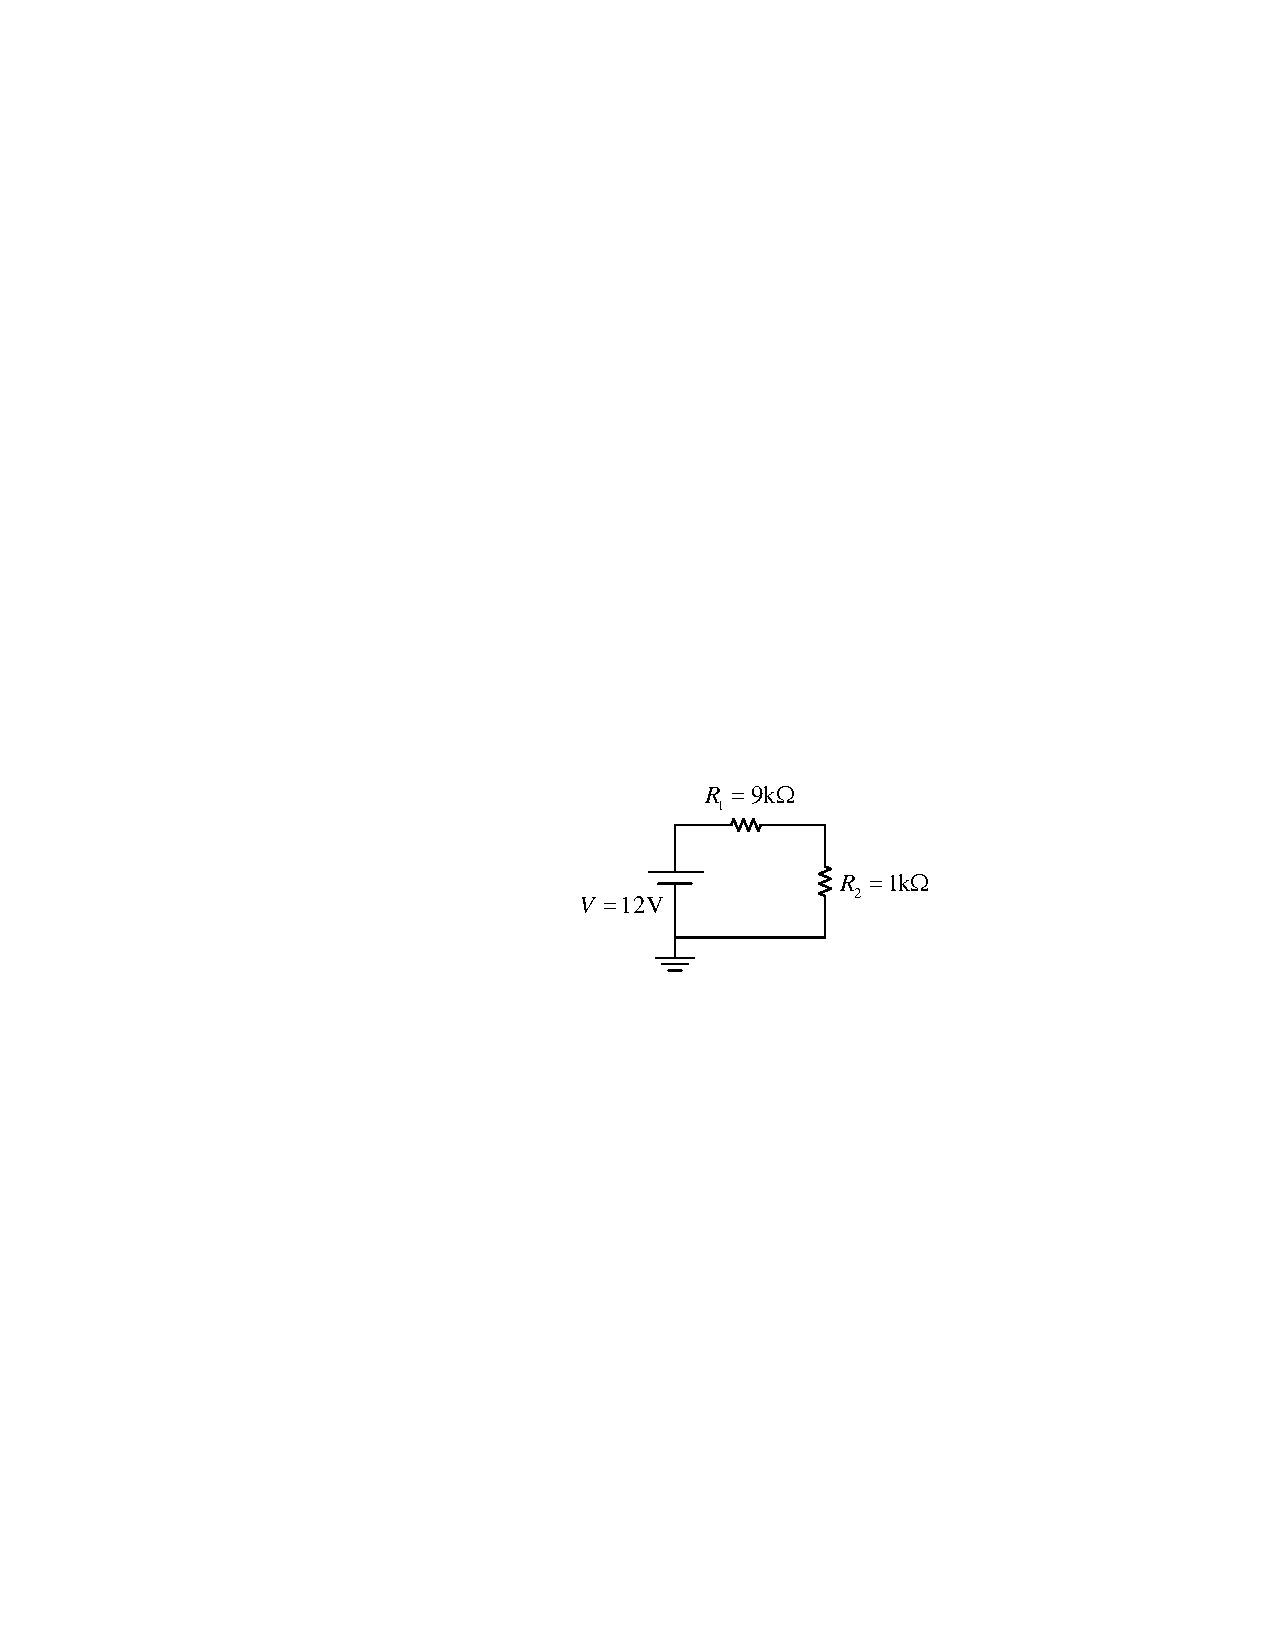
\includegraphics[scale=1.2,angle=0]{Fig/cir1.pdf}
        \caption{A voltage divider circuit.} \label{fig:cir1}
    \end{figure}

    %--------------------------------------------
    \begin{subquestion}{Build the circuit on a breadboard. Can you find a $9$ k$\Omega$ resistor in the stackable element storage box? }
        \answer{
            We used two parallel $18k\Omega$ resistors to obtain $9k\Omega$.
            The $9k\Omega$ resistor is not available in the stackable element storage box since
            it's not a standard value in the E12 series.

        }
    \end{subquestion}

    %--------------------------------------------
    \begin{subquestion}{Which resistor is a suitable replacement for a $9$ k$\Omega$ resistor? Pick that resistor and read its color code.}
        \answer{
            We used two parallel $18k\Omega$ resistors to obtain $9k\Omega$. We could also use an $8k\Omega$ because E12 resistors have $5\%$ error.
        }
    \end{subquestion}

    %--------------------------------------------
    \begin{subquestion}{Measure the voltage across each resistor. Is there any difference between the measured and analytical values?}
        \answer{
            \begin{figure}[H]
                \centering
                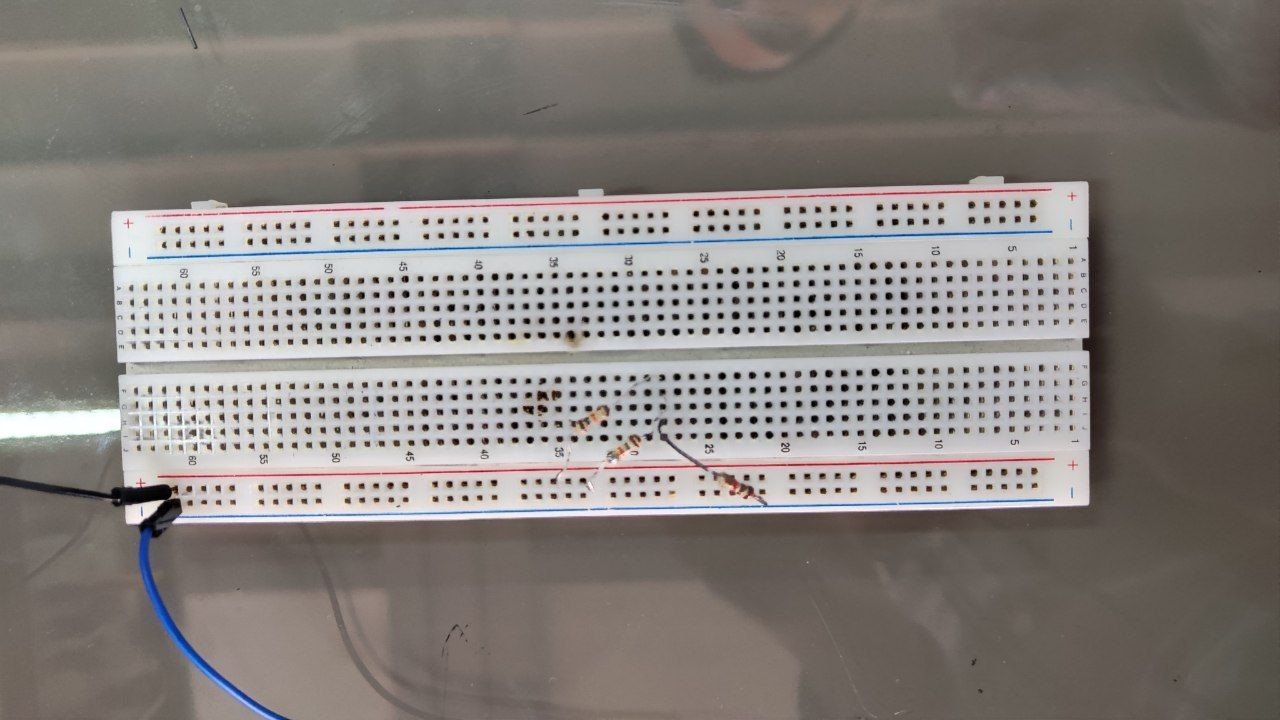
\includegraphics[scale=\PicScale,angle=0]{Fig/1.jpeg}
                \caption{The circuit.}
            \end{figure}
            \begin{figure}[H]
                \centering
                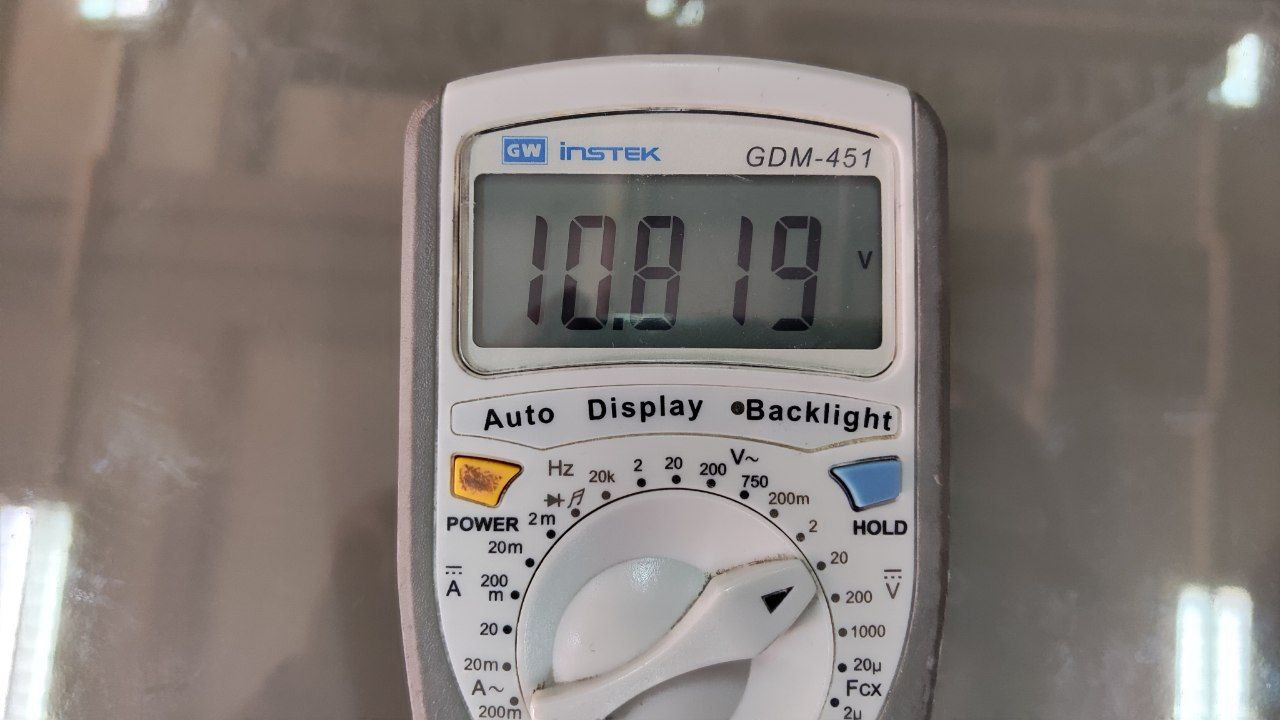
\includegraphics[scale=0.12,angle=0]{Fig/2.jpeg}
                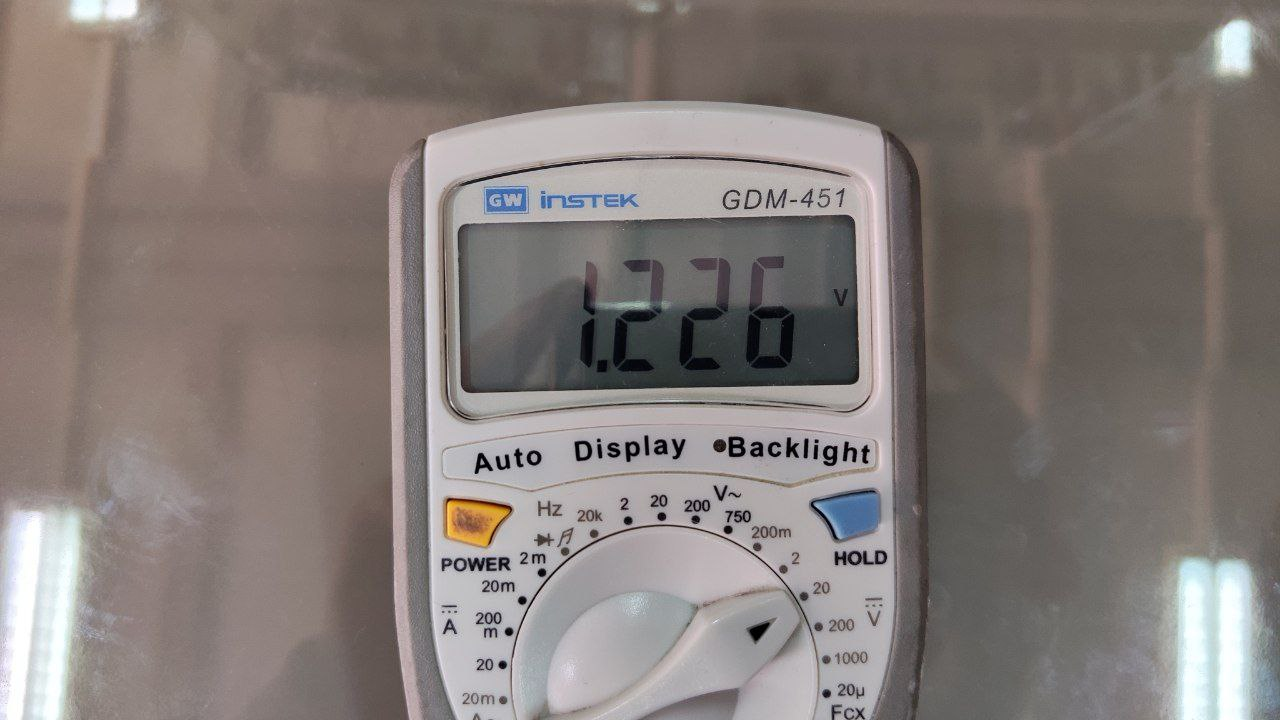
\includegraphics[scale=0.12,angle=0]{Fig/3.jpeg}
                \caption{measured voltage value.}
            \end{figure}

            Yes, there is a difference between the values and the reason is
            the tolerance of the resistors.
        }
    \end{subquestion}

\end{question}


%----------------------------------------------------------------------------------------
%	QUESTION 2
%----------------------------------------------------------------------------------------

\begin{question}

    \questiontext{Each real circuit element has a nominal value within a tolerance band.}

    %--------------------------------------------
    \begin{subquestion}{Pick up ten E12 $1$ k$\Omega$ resistors and measure their resistance. Calculate the maximum, minimum, mean, variance, and standard deviation of the measured values and interpret them considering the nominal and tolerance values. }
        \answer{
            We used E24 resistors instead. \\
            values: $1.0103, 0.9940, 1.0027, 1.0018, 1.0012, 1.0015, 0.9964, 0.9996, 0.9979$ and $1.0135~k\Omega$.
        }
    \end{subquestion}

    %--------------------------------------------
    \begin{subquestion}{Repeat the previous part for ten E12 $10$ $\mu$F capacitors. }
        \answer{
            values: $9.76, 9.64, 9.05, 9.49, 9.19, 9.32, 9.61, 9.73, 9.37$ and $9.31~\mu F$
        }
    \end{subquestion}

\end{question}

%----------------------------------------------------------------------------------------
%	QUESTION 3
%----------------------------------------------------------------------------------------

\begin{question}

    \questiontext{\underline{This experiment should be done by the lab supervisor}. Dependency of the value of a real circuit element on temperature is characterized by a specified temperature coefficient. }

    %--------------------------------------------
    \begin{subquestion}{Measure the resistance of a carbon resistor in room temperature. Redo the measurement when the resistor is heated by a soldering iron and when is cooled by a cooling spray. }
        \answer{
            This part was done by the lab supervisor.
        }
    \end{subquestion}

    %--------------------------------------------
    \begin{subquestion}{Repeat the previous part for a metal film resistor, a ceramic capacitor, and a multi-layer capacitor. }
        \answer{
            This part was done by the lab supervisor.
        }
    \end{subquestion}

\end{question}

%----------------------------------------------------------------------------------------
%	QUESTION 4
%----------------------------------------------------------------------------------------

\begin{question}

    \questiontext{\underline{This experiment should be done by the lab supervisor}. Each resistor has a specific maximum power rating. Connect a $0.25$ W $10$ $\Omega$ resistor to a DC power supply using an alligator clip wire. Sweep the voltage from $0$ to $5$ V and observe the results.}

    \answer{
        This part was done by the lab supervisor. When a $0.25$ W, $10$ $\Omega$ resistor is connected to a DC power supply
        and the voltage is swept from $0$ to $5$ V, the current through
        the resistor increases linearly with the voltage, as per
        Ohm's law ($I = \frac{V}{R}$).

        However, the power dissipated by the resistor,
        given by $P = IV = V^2/R$, also increases with the square
        of the voltage. If the power exceeds the resistor's power
        rating of $0.25$ W, the resistor can overheat and potentially
        fail.

        In this case, at $5$ V, the power dissipated by the resistor
        would be $P = V^2/R = 5^2/10 = 2.5$ W, which exceeds the
        resistor's power rating.
    }
\end{question}

%----------------------------------------------------------------------------------------
%	QUESTION 4
%----------------------------------------------------------------------------------------

\begin{question}

    \questiontext{\underline{This experiment should be done by the lab supervisor}. Each capacitor has a specific maximum voltage. Further, a capacitor may have a  specific voltage polarity. }

    %--------------------------------------------
    \begin{subquestion}{Connect a $16$ V aluminum electrolytic capacitor directly to a $30$ V DC voltage and observe the results.}
        \answer{
            \begin{figure}[H]
                \centering
                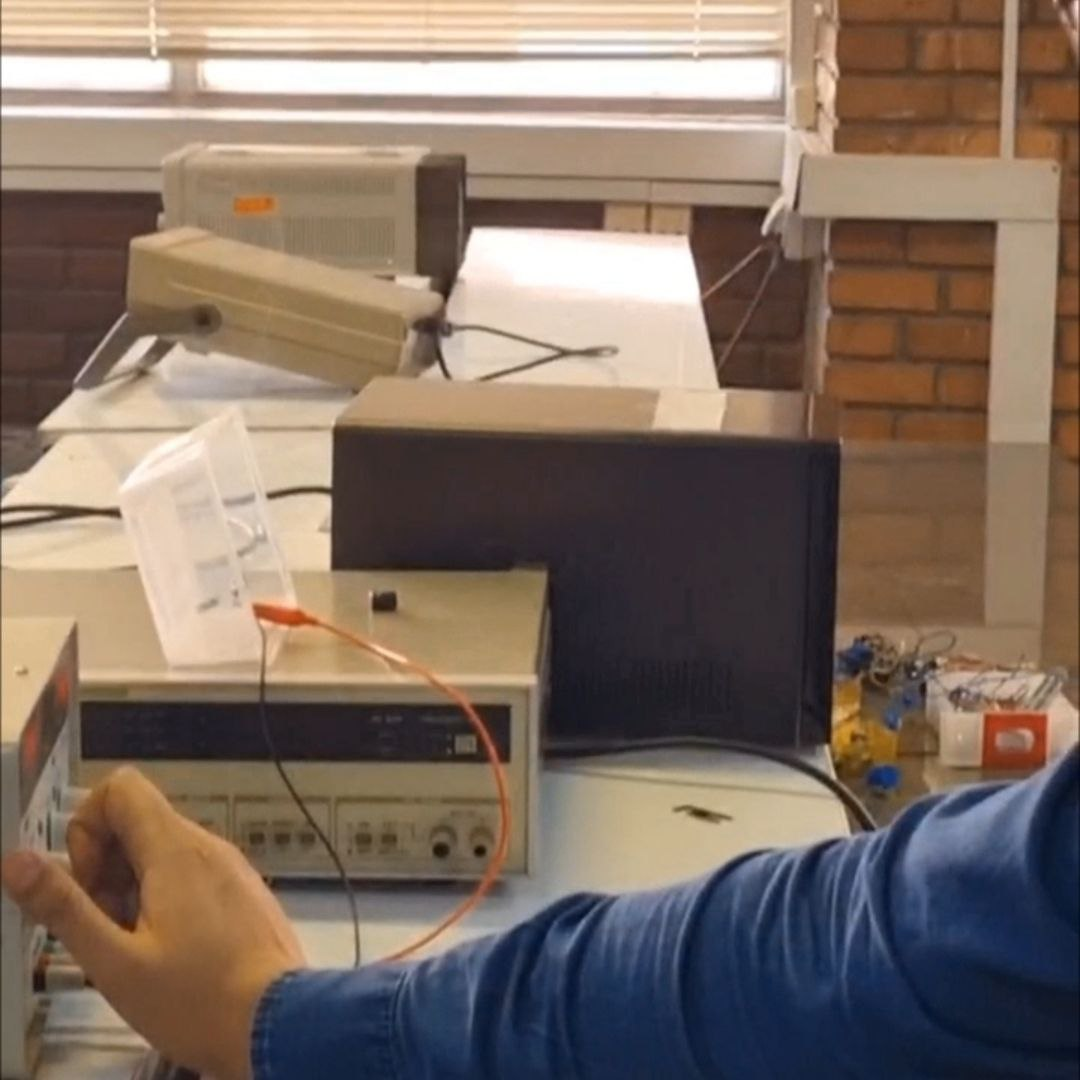
\includegraphics[scale=0.08,angle=0]{Fig/4.jpeg}
                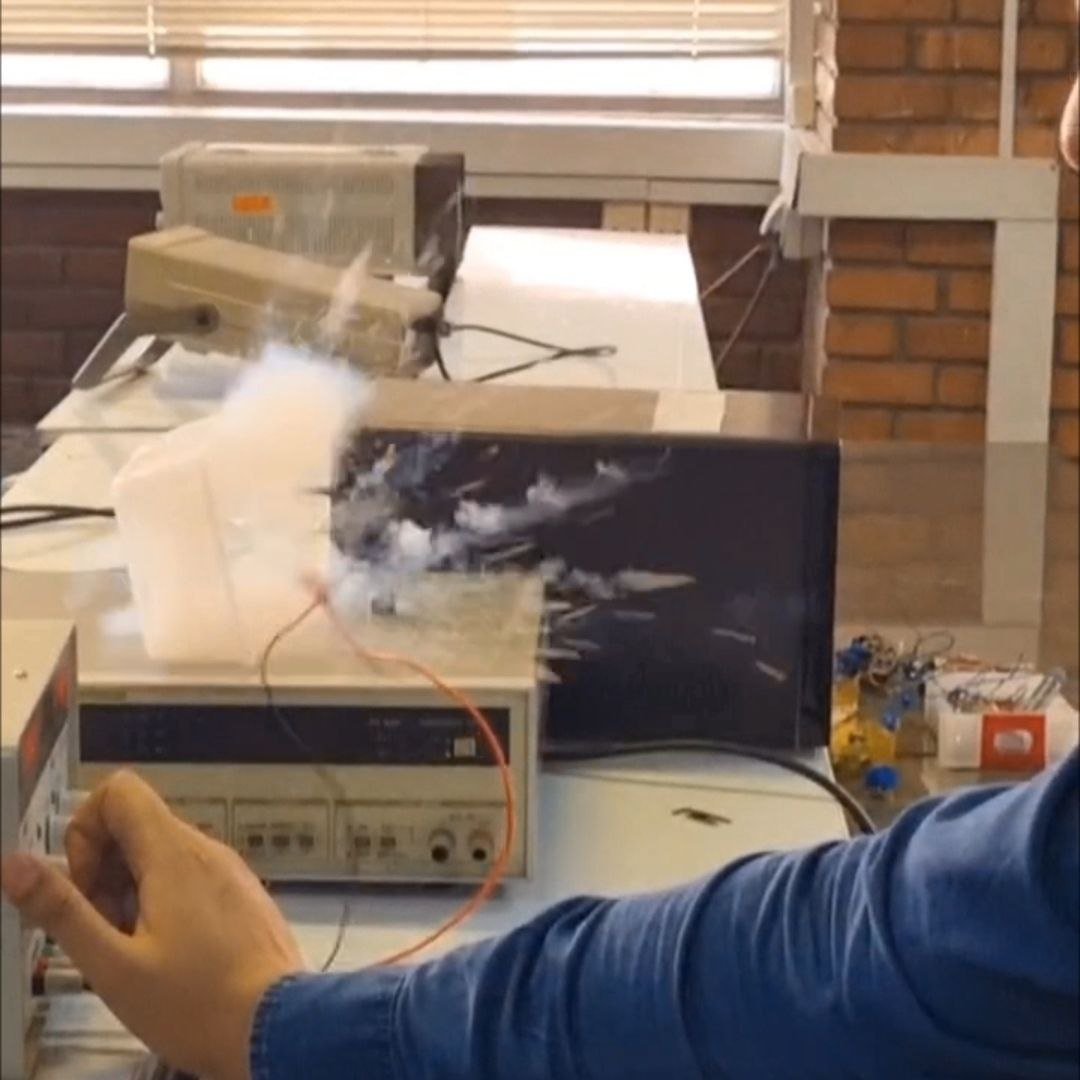
\includegraphics[scale=0.08,angle=0]{Fig/5.jpeg}
                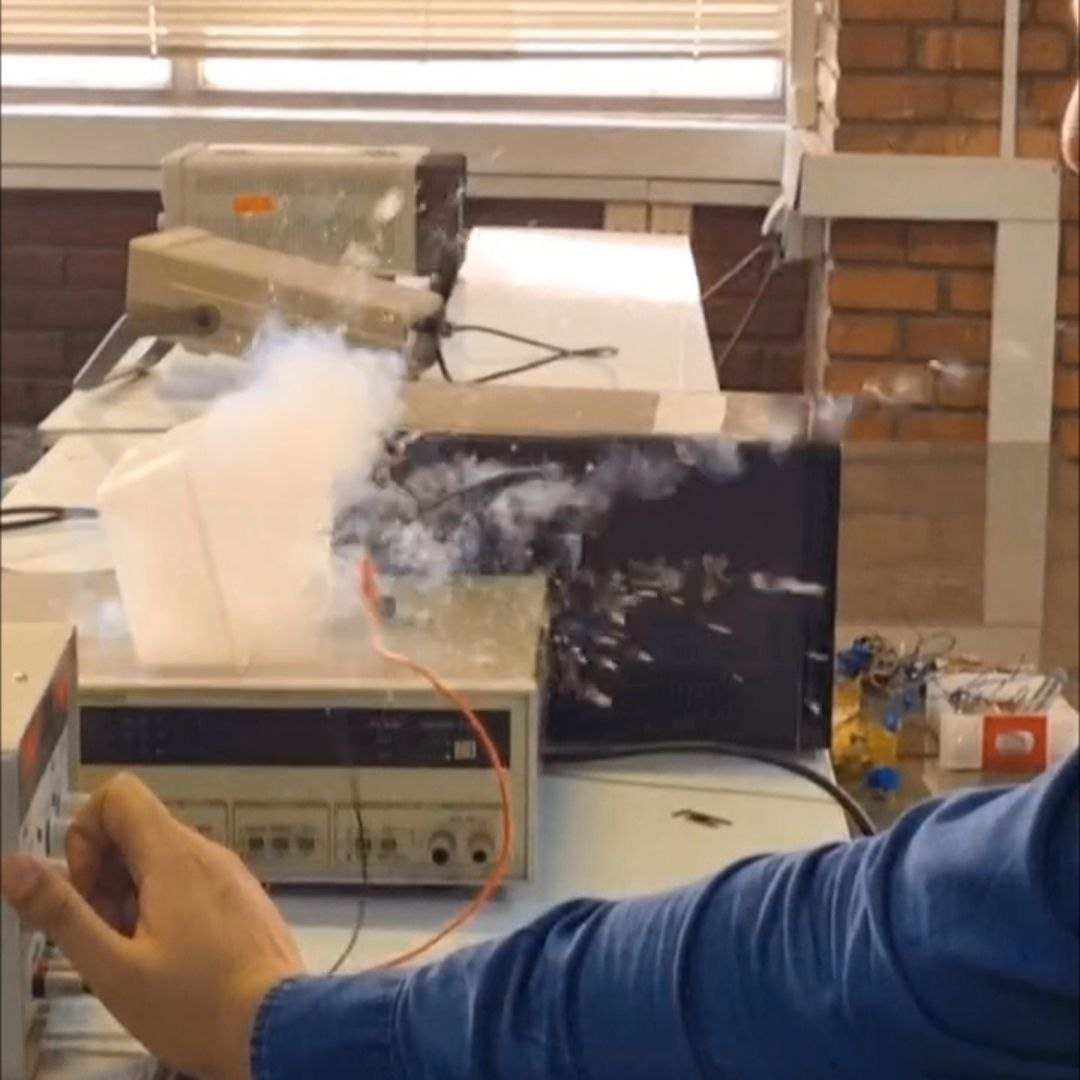
\includegraphics[scale=0.08,angle=0]{Fig/6.jpeg}
                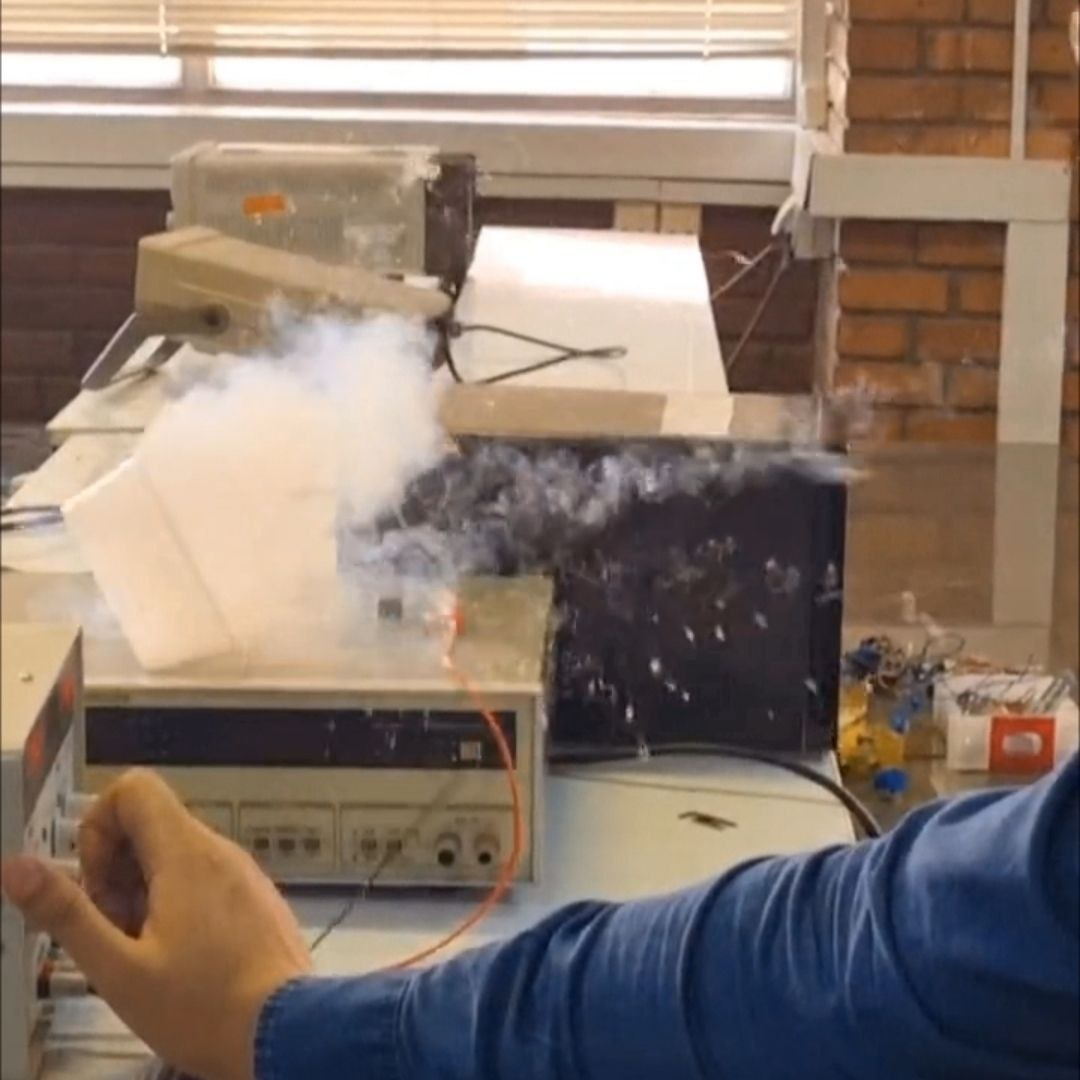
\includegraphics[scale=0.08,angle=0]{Fig/7.jpeg}
            \end{figure}

            This part was done by the lab supervisor. As can be seen, whn a $16$ V aluminum electrolytic capacitor is connected
            directly to a $30$ V DC voltage, it exceeds the capacitor's rated maximum voltage.
            This can lead to a breakdown of the dielectric material inside the capacitor, causing capacitor failure(explosion).
        }
    \end{subquestion}

    %--------------------------------------------
    \begin{subquestion}{Connect a $16$ V aluminum electrolytic capacitor inversely to a $16$ V DC voltage and observe the results.}
        \answer{
            This part was done by the lab supervisor. When a $16$ V aluminum electrolytic capacitor is connected inversely
            (i.e., with reversed polarity) to a $16$ V DC voltage, it can also lead to a breakdown. Electrolytic capacitors are polarized,
            meaning they have a positive and a negative terminal. If they are connected in reverse, the oxide layer on the anode,
            which acts as the dielectric, can break down, leading to a short circuit. This can cause the capacitor to heat up,
            potentially leading to an explosion or leakage of the electrolyte.
            In short, although the voltage limit is not exceeded, the polarity of the capacitor must be observed to prevent damage.
        }
    \end{subquestion}


\end{question}

%----------------------------------------------------------------------------------------
%	QUESTION 1
%----------------------------------------------------------------------------------------

\begin{question}

    \questiontext{Build the circuit shown in Fig. \ref{fig:cir2} on a breadboard, where $r=1$ k$\Omega$ denotes a resistor allowing to measure the current indirectly.}

    \begin{figure}[H]
        \centering
        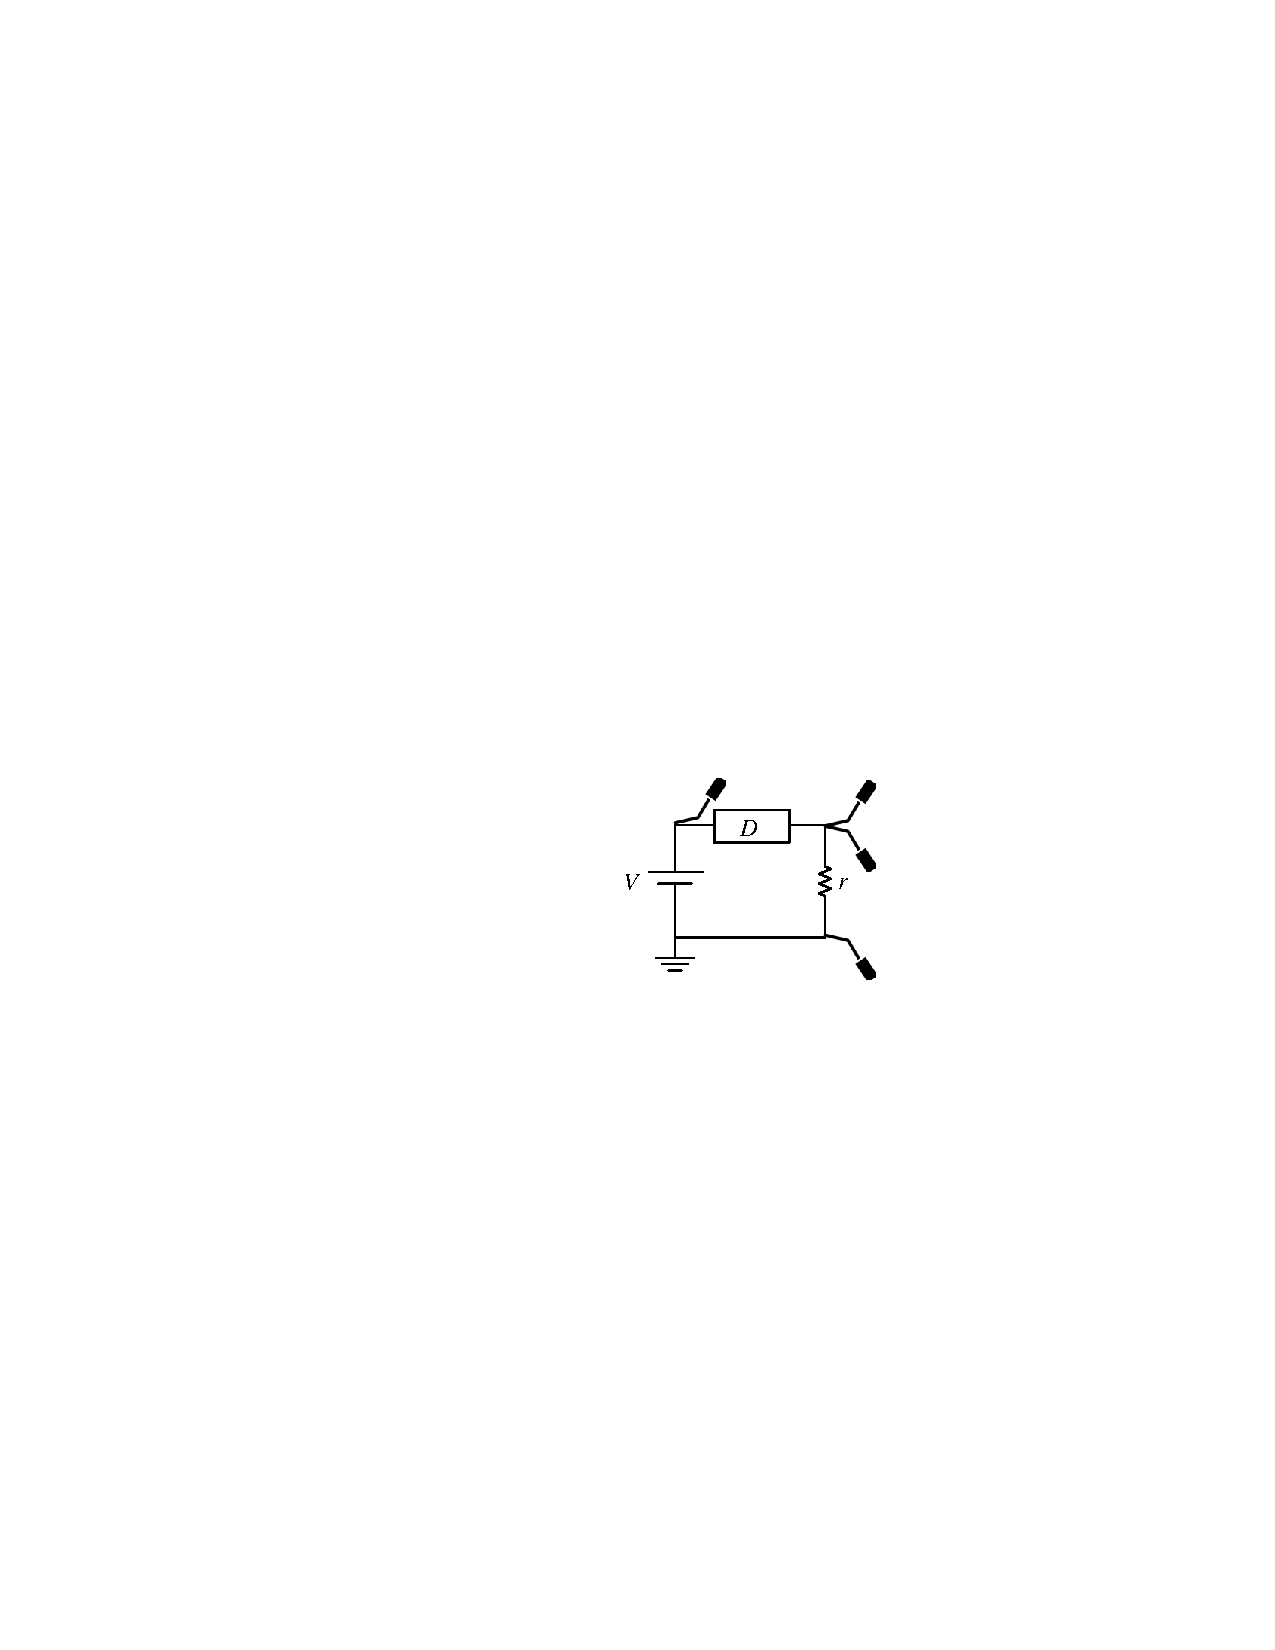
\includegraphics[scale=1.2,angle=0]{Fig/cir2.pdf}
        \caption{A test circuit for extracting the characteristic curve of a resistive element using multimeter.} \label{fig:cir2}
    \end{figure}

    %--------------------------------------------
    \begin{subquestion}{Replace $D$ with a $1$ k$\Omega$ resistor. Sweep the DC voltage over negative and positive ranges and record the voltage and current of the resistor using a multimeter. Use the recorded data to plot the characteristic curve of the resistor.}
        \answer{
            \begin{figure}[H]
                \centering
                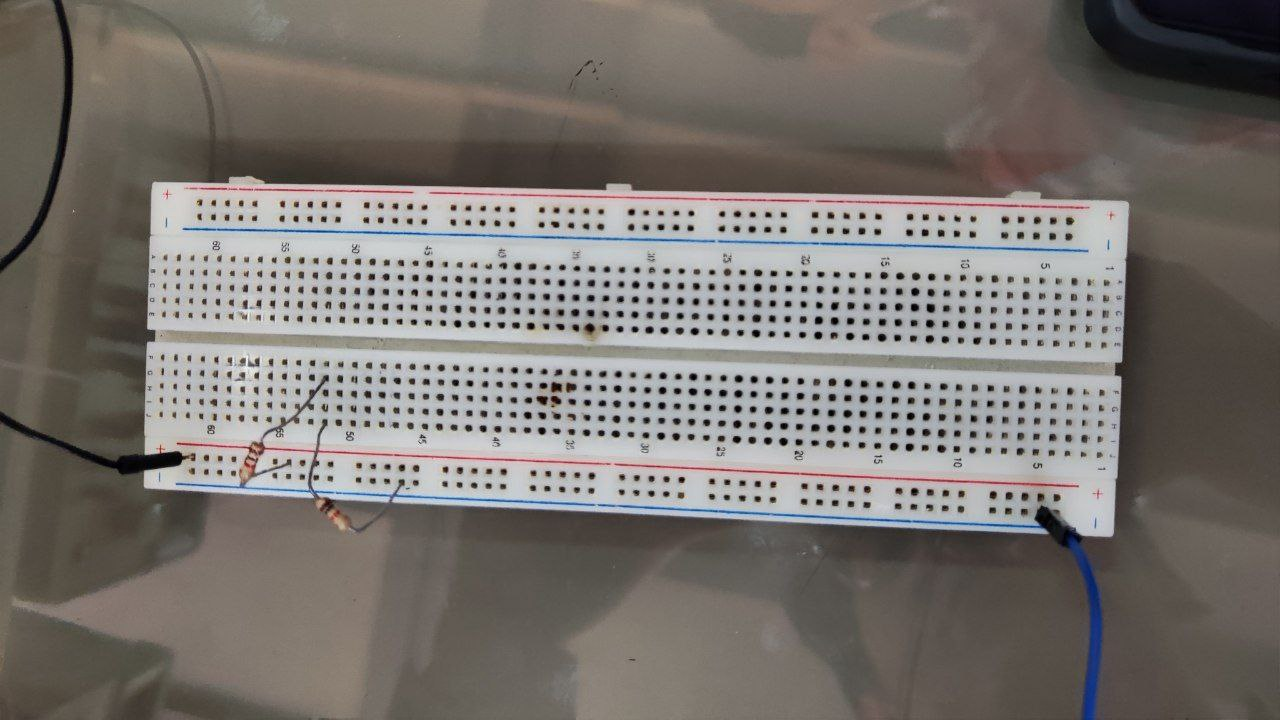
\includegraphics[scale=\PicScale,angle=0]{Fig/8.jpeg}
                \caption{The circuit.}
            \end{figure}

            \begin{figure}[H]
                \centering
                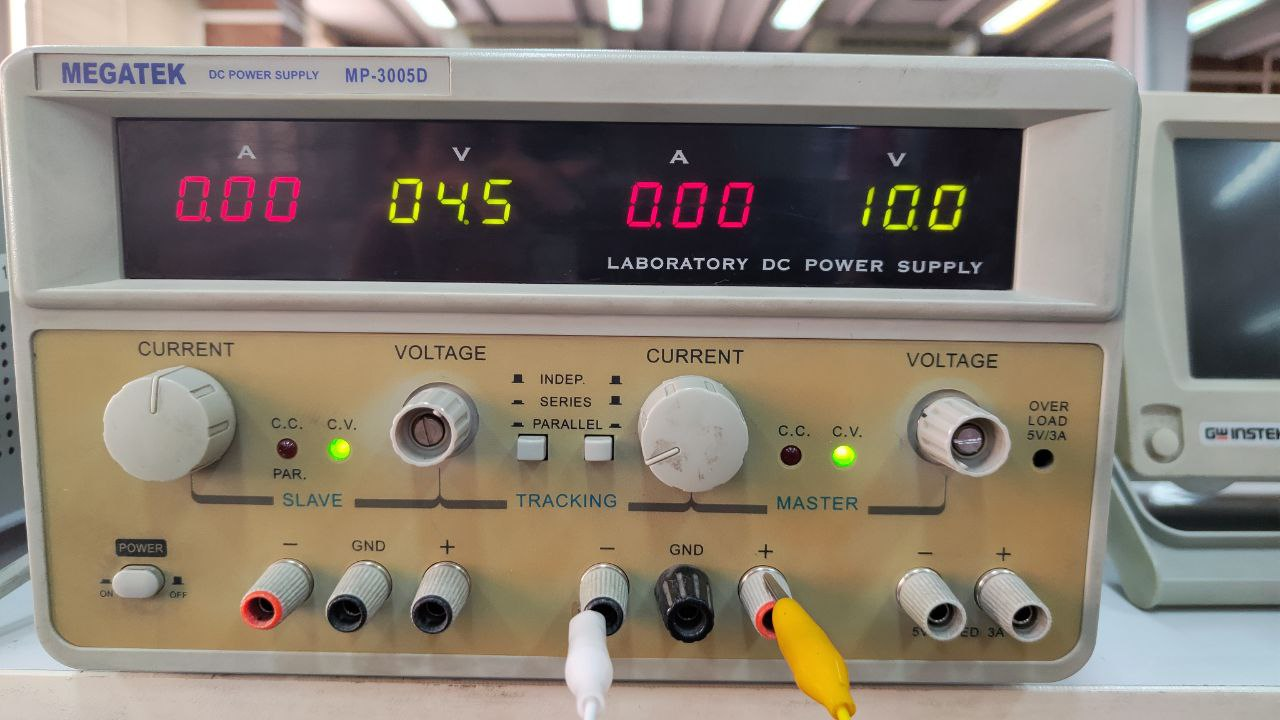
\includegraphics[scale=\PicScale,angle=0]{Fig/9.jpeg}
                \caption{DC power supply set to $10V$ and $-10V$.}
            \end{figure}
            \begin{figure}[H]
                \centering
                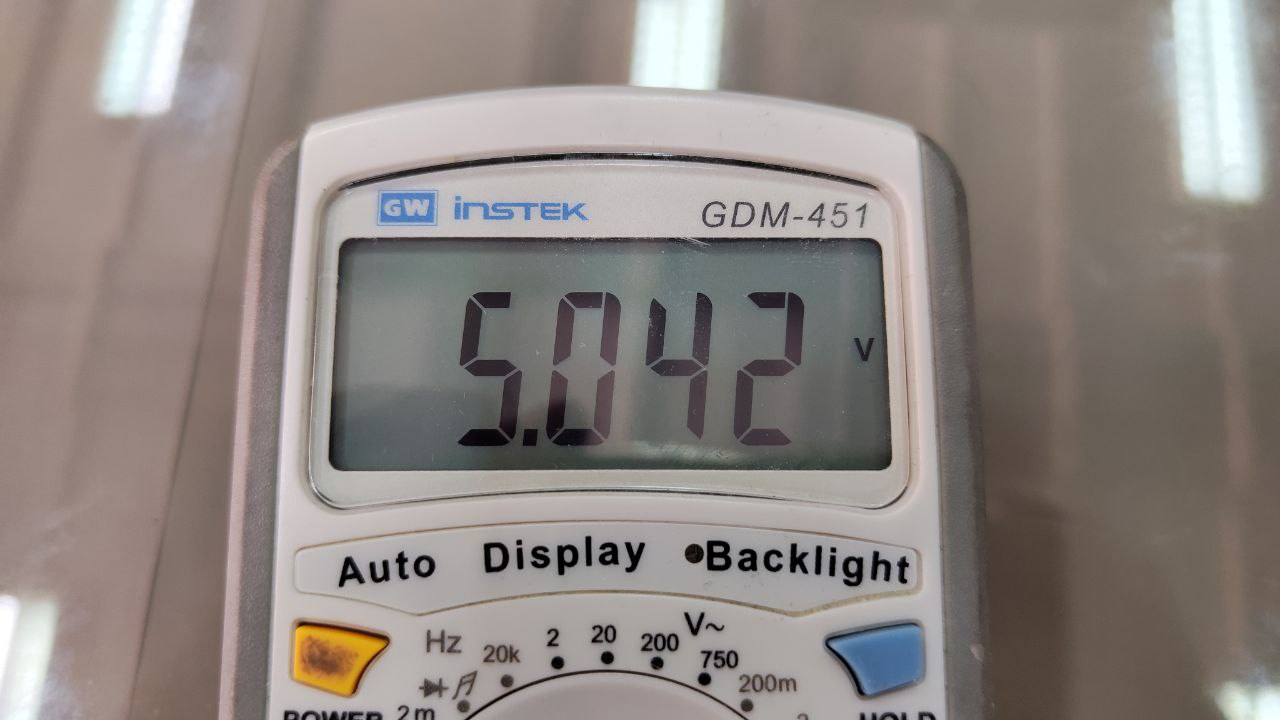
\includegraphics[scale=0.08,angle=0]{Fig/10.jpeg}
                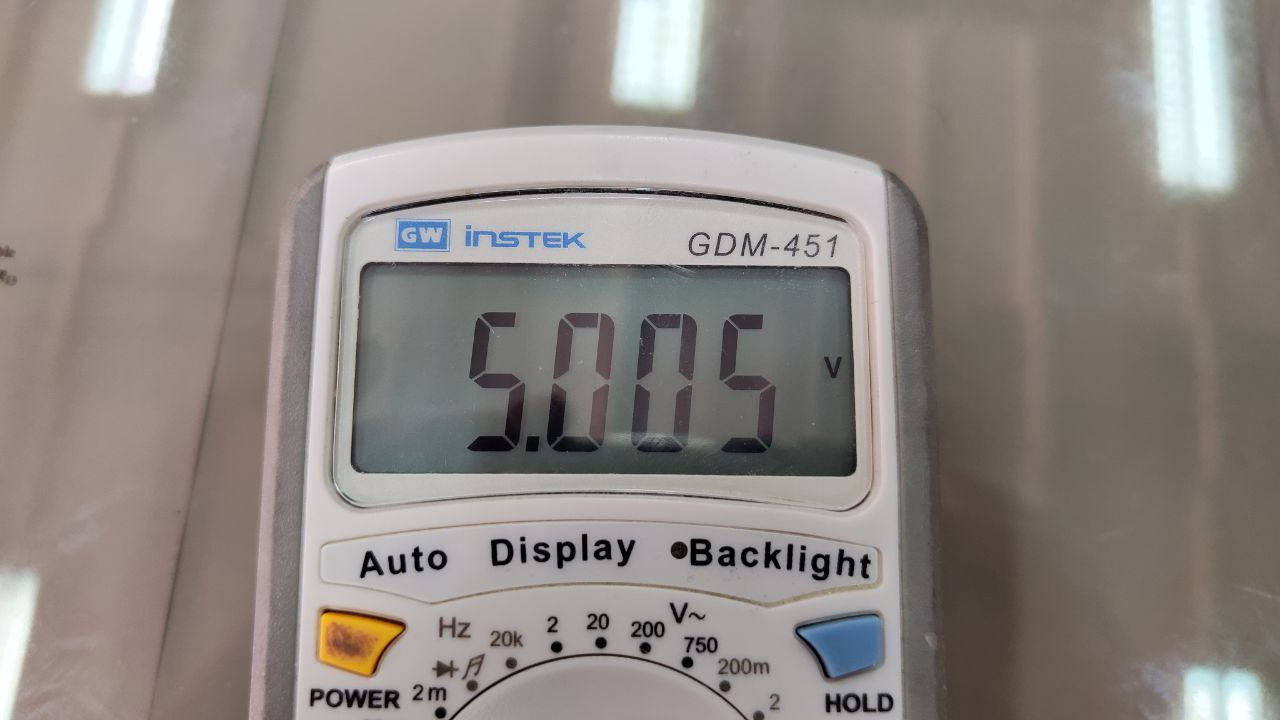
\includegraphics[scale=0.08,angle=0]{Fig/11.jpeg}
                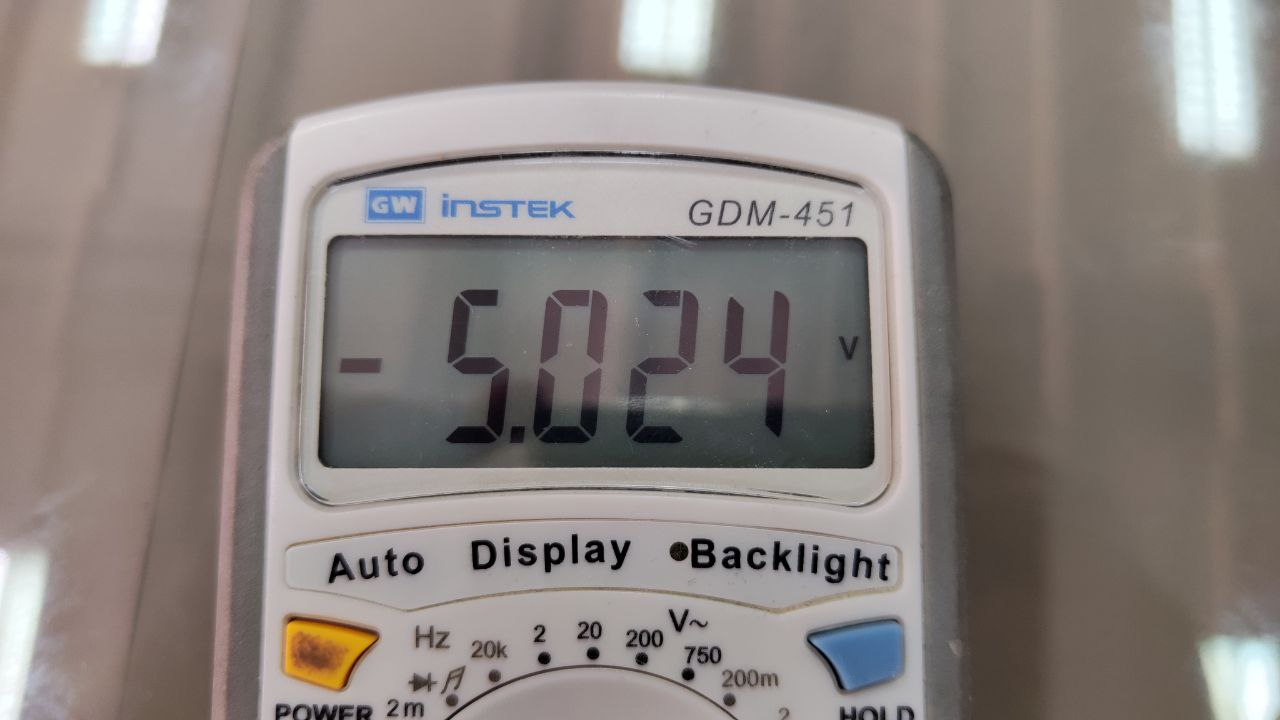
\includegraphics[scale=0.08,angle=0]{Fig/12.jpeg}
                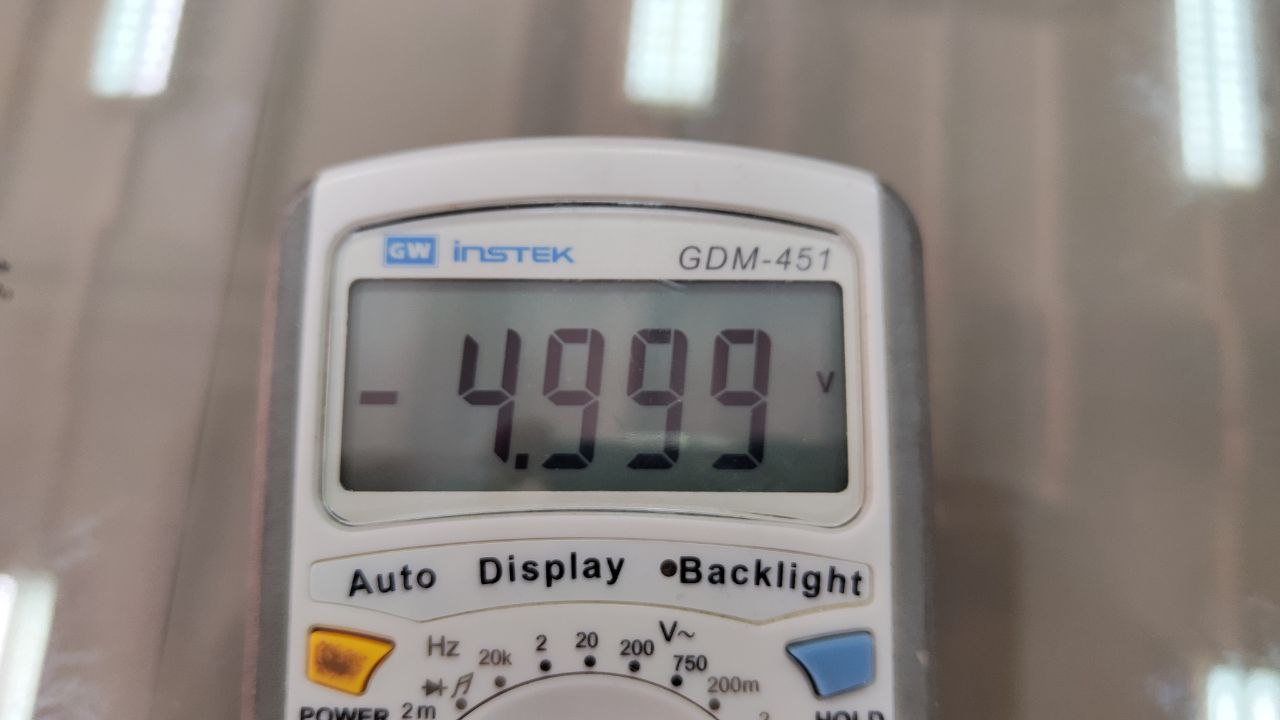
\includegraphics[scale=0.08,angle=0]{Fig/13.jpeg}
                \caption{First image is for D and $10V$, second image is for r and $10V$. \\
                    \hspace*{14mm} Third image is for D and $-10V$, last image is for r and $-10V$.}
            \end{figure}
            \begin{figure}[H]
                \centering
                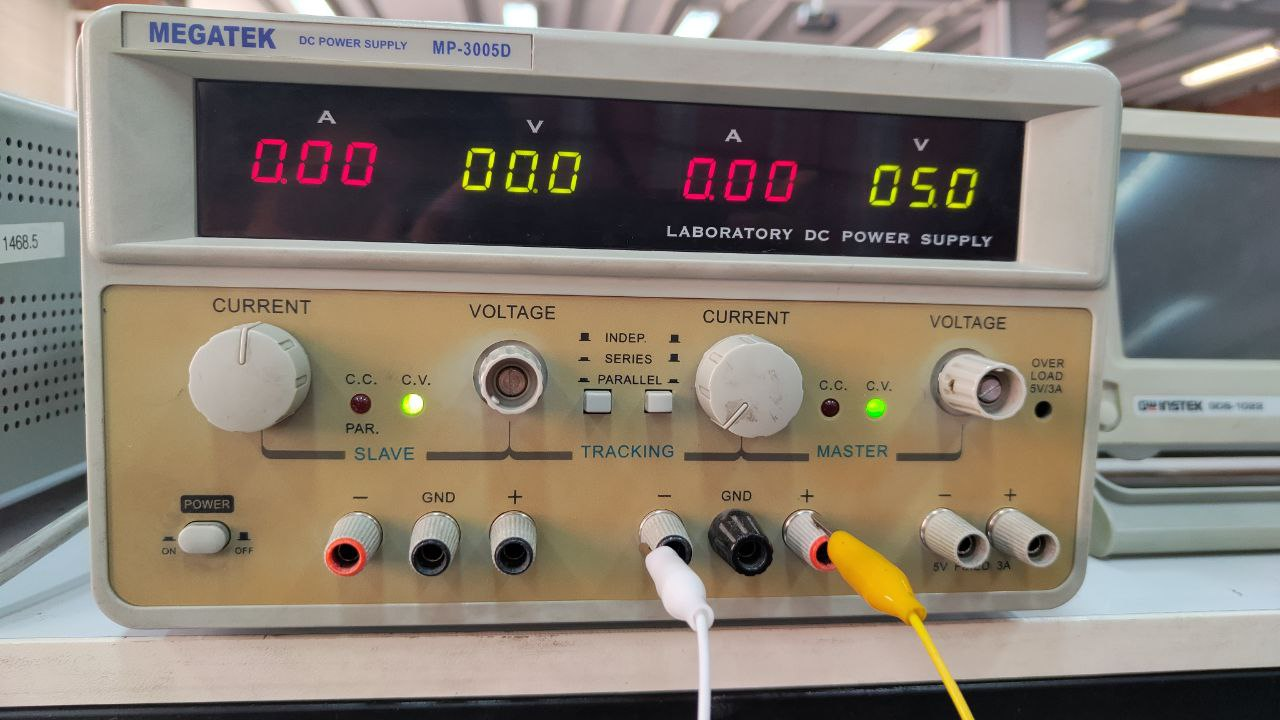
\includegraphics[scale=\PicScale,angle=0]{Fig/14.jpeg}
                \caption{DC power supply set to $5V$ and $-5V$.}
            \end{figure}
            \begin{figure}[H]
                \centering
                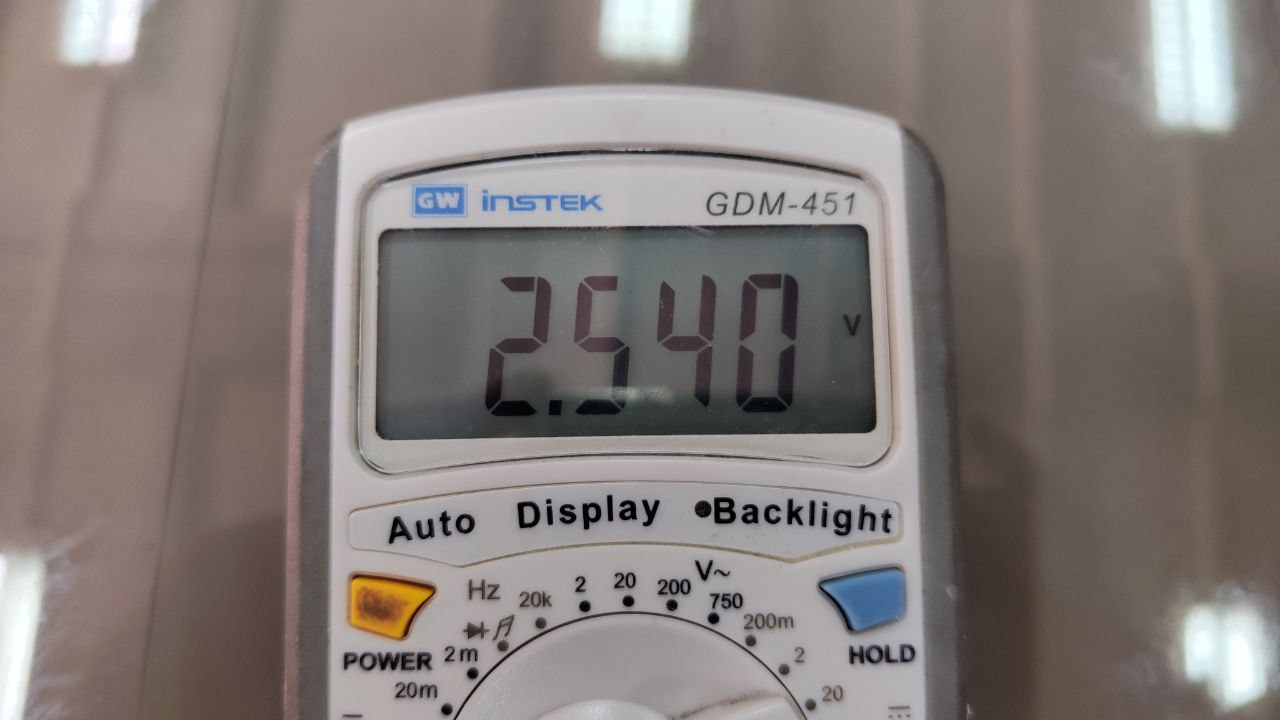
\includegraphics[scale=0.08,angle=0]{Fig/15.jpeg}
                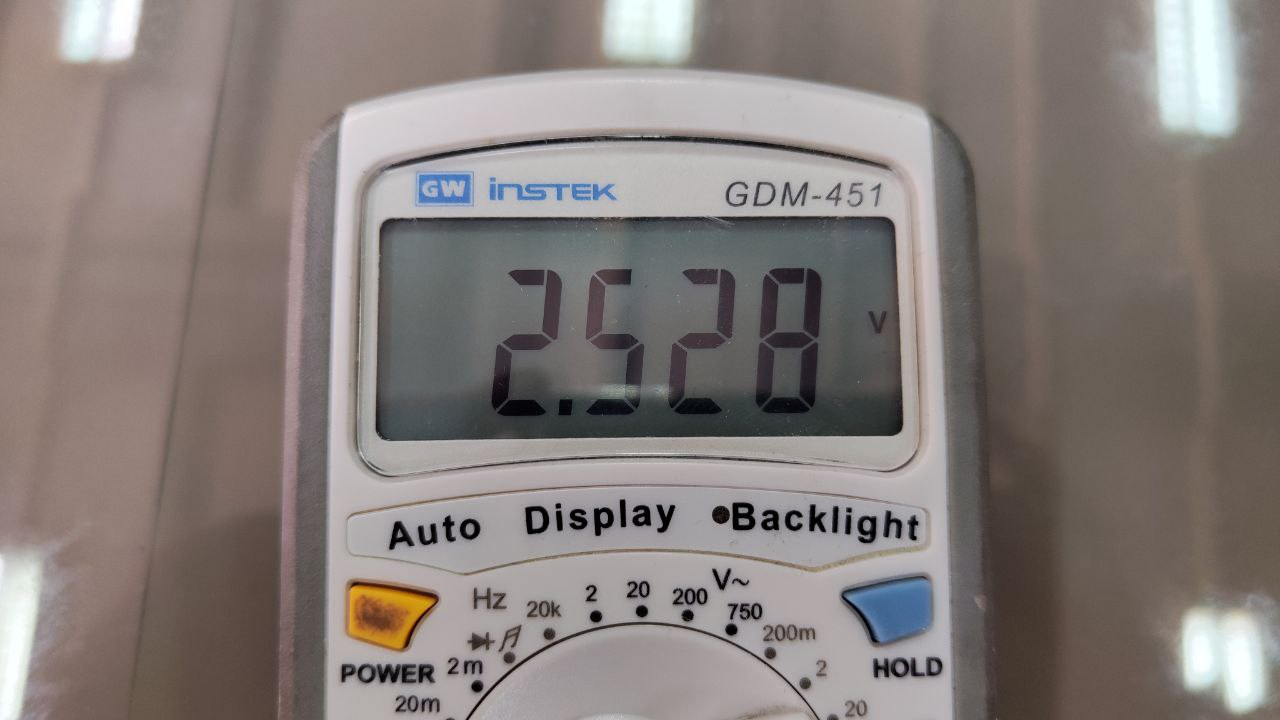
\includegraphics[scale=0.08,angle=0]{Fig/16.jpeg}
                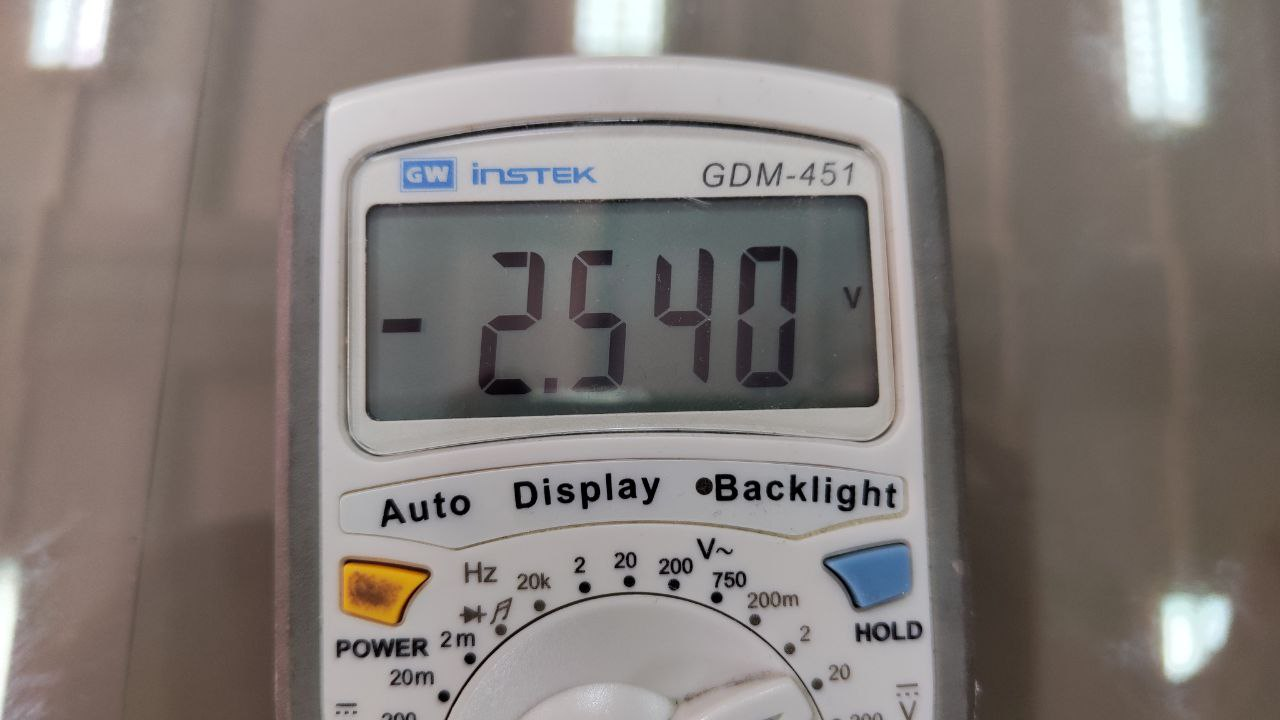
\includegraphics[scale=0.08,angle=0]{Fig/17.jpeg}
                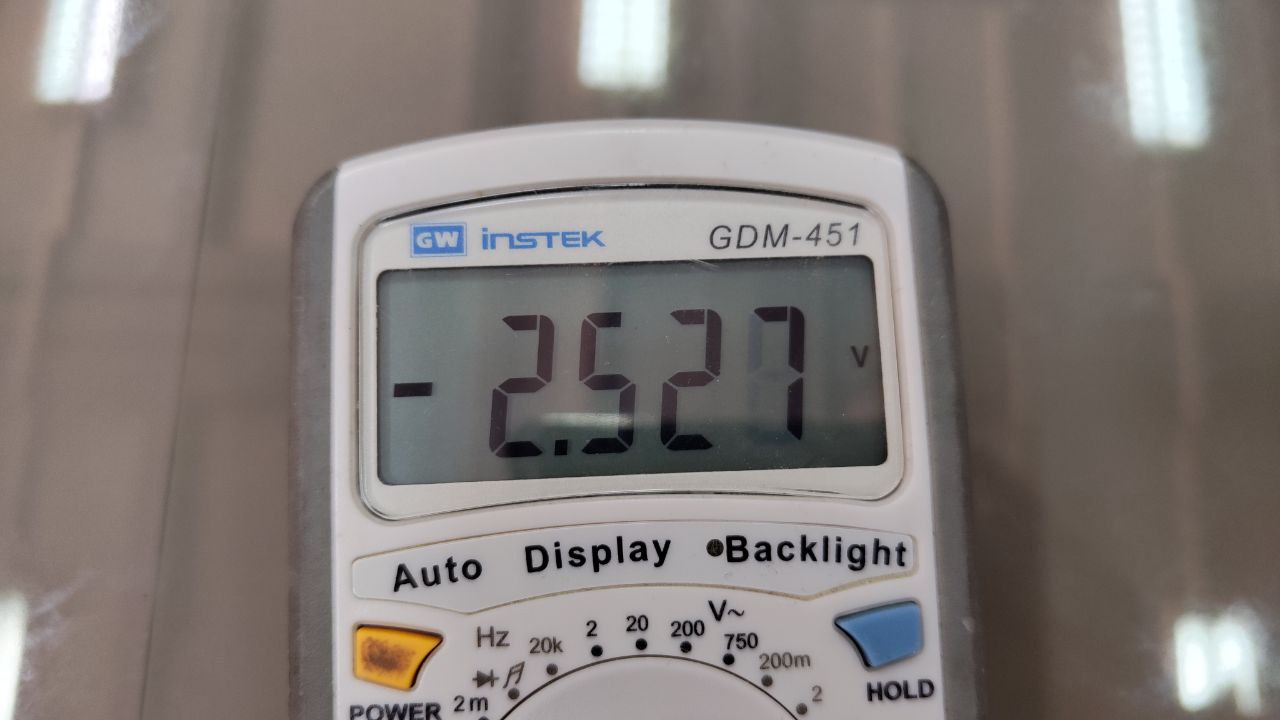
\includegraphics[scale=0.08,angle=0]{Fig/18.jpeg}
                \caption{First image is for D and $5V$, second image is for r and $5V$. \\
                    \hspace*{14mm} Third image is for D and $-5V$, last image is for r and $-5V$.}
            \end{figure}
            \begin{figure}[H]
                \centering
                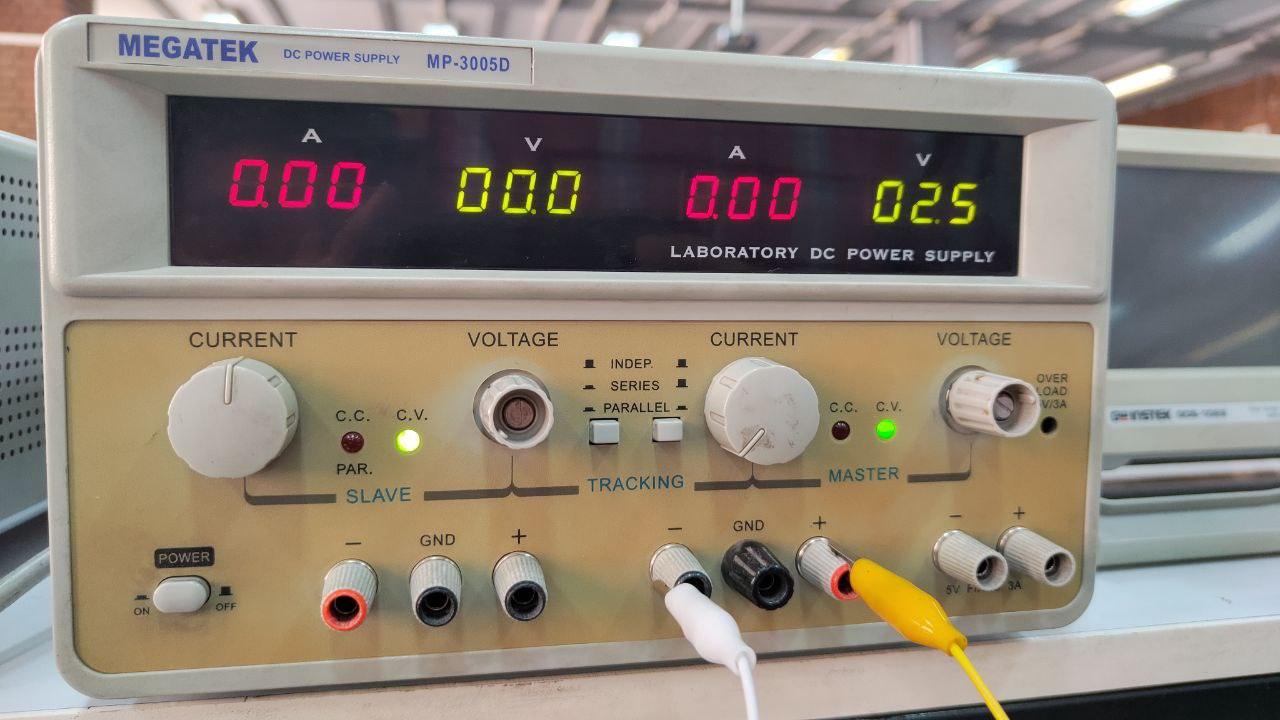
\includegraphics[scale=\PicScale,angle=0]{Fig/19.jpeg}
                \caption{DC power supply set to $2.5V$ and $-2.5V$.}
            \end{figure}
            \begin{figure}[H]
                \centering
                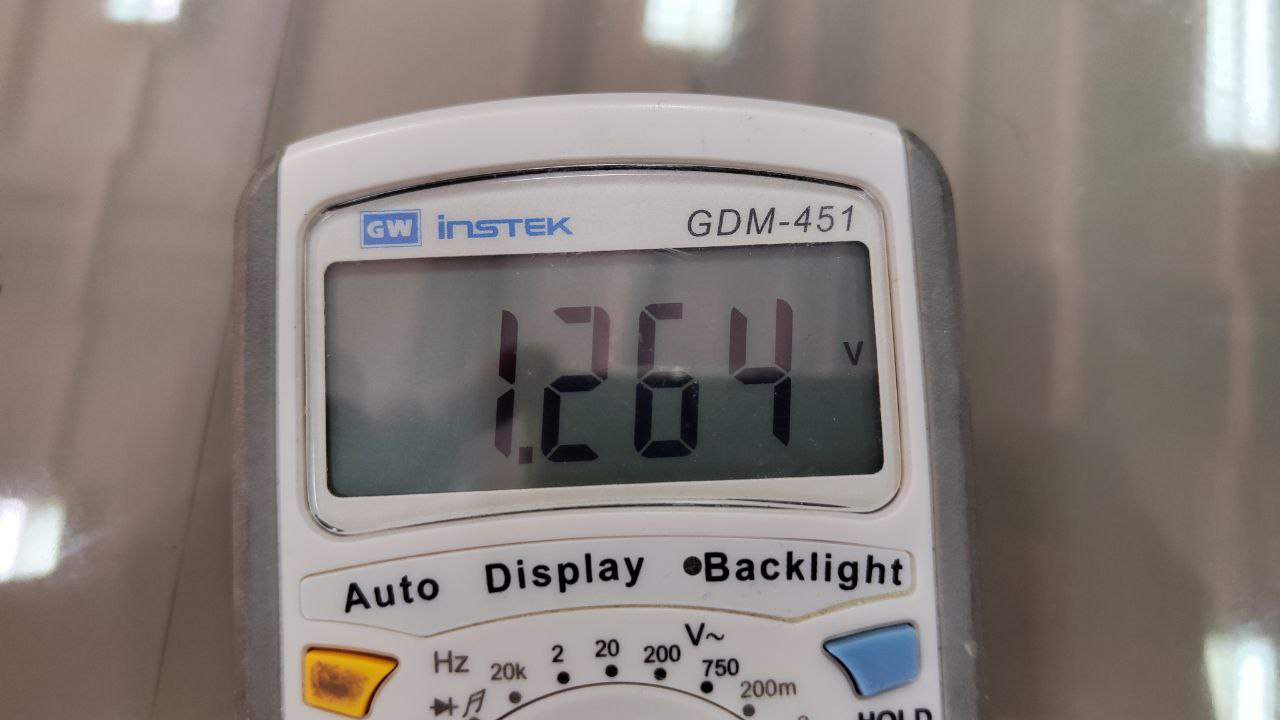
\includegraphics[scale=0.08,angle=0]{Fig/20.jpeg}
                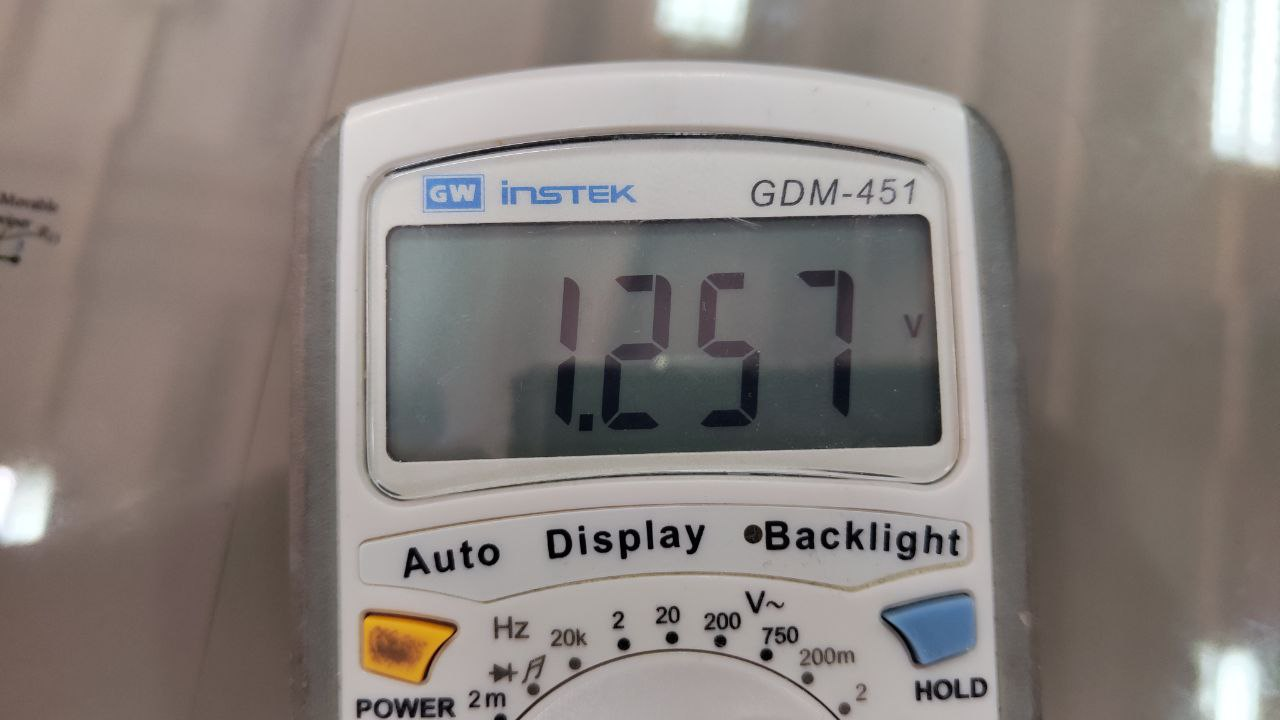
\includegraphics[scale=0.08,angle=0]{Fig/21.jpeg}
                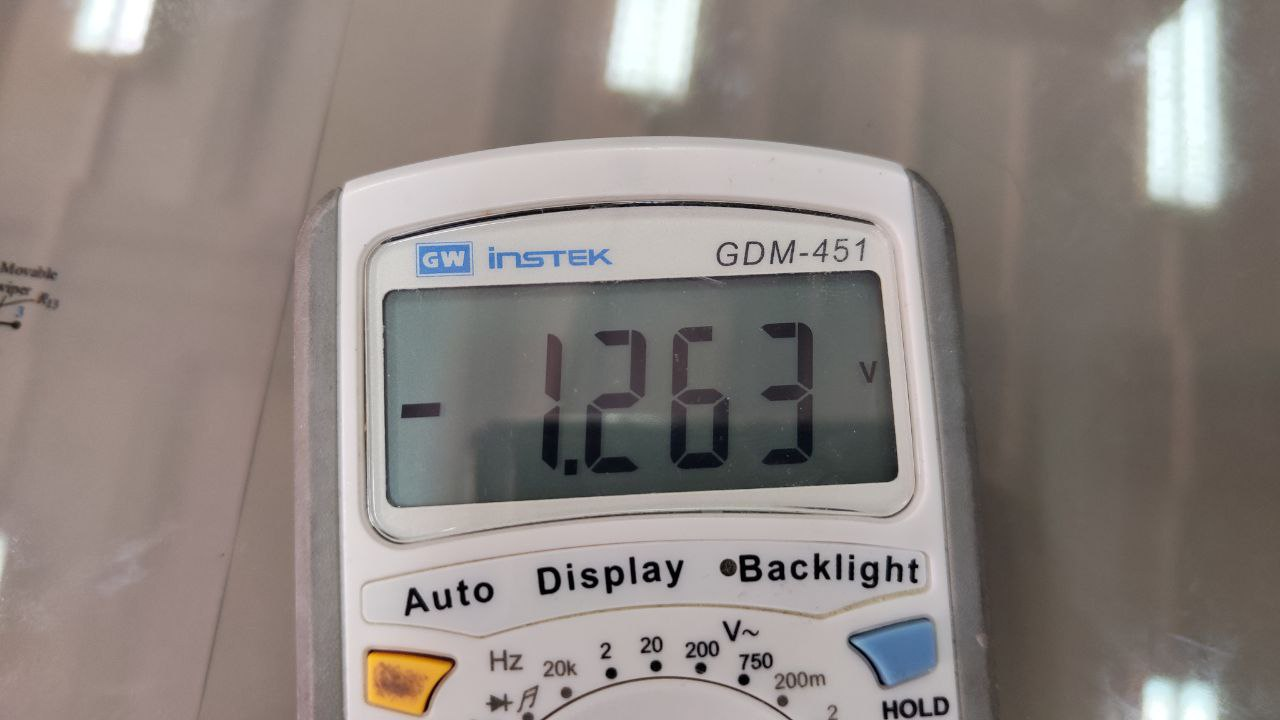
\includegraphics[scale=0.08,angle=0]{Fig/22.jpeg}
                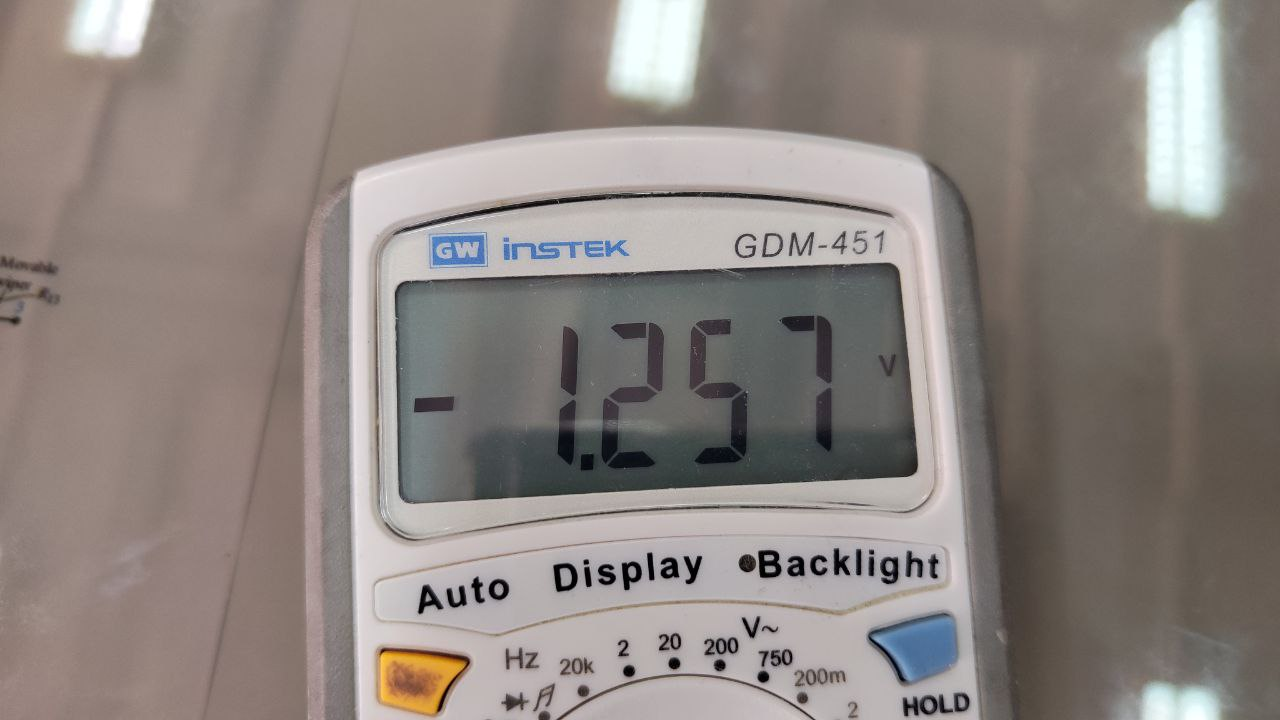
\includegraphics[scale=0.08,angle=0]{Fig/23.jpeg}
                \caption{First image is for D and $2.5V$, second image is for r and $2.5V$. \\
                    \hspace*{14mm} Third image is for D and $-2.5V$, last image is for r and $-2.5V$.}
            \end{figure}

            The points for D element are:
            \begin{table}[H]
                \centering
                \begin{tabular}{|c|c|c|c|c|c|c|c|c|c|c|}
                    \hline
                    $V$   & $-10$   & $-5$    & $-2.5$  & $0$ & $2.5$  & $5$    & $10$   \\ \hline
                    $V_d$ & $-5.02$ & $-2.54$ & $-1.26$ & $0$ & $1.26$ & $2.54$ & $5.04$ \\ \hline
                \end{tabular}
            \end{table}

            The exact value of r resistance was $0.991k\Omega$ (using a multimeter).
            Using the Ohm's law, we can calculate the current flowing through the circuit, and then,
            since we already know the voltage of D element, we can plot the characteristic curve of the D element.
            The points $(V,V_r)$ for r resistor are:
            \begin{table}[H]
                \centering
                \begin{tabular}{|c|c|c|c|c|c|c|c|c|c|c|}
                    \hline
                    $V$   & $-10$   & $-5$    & $-2.5$  & $0$ & $2.5$  & $5$    & $10$   \\ \hline
                    $V_r$ & $-4.99$ & $-2.52$ & $-1.25$ & $0$ & $1.25$ & $2.52$ & $5.00$ \\ \hline
                \end{tabular}
            \end{table}

            So the current flowing through the circuit based on V is:
            \begin{table}[H]
                \centering
                \begin{tabular}{|c|c|c|c|c|c|c|c|c|c|c|}
                    \hline
                    $V$ & $-10$     & $-5$      & $-2.5$    & $0$ & $2.5$    & $5$      & $10$     \\ \hline
                    $I$ & $-5.00mA$ & $-2.52mA$ & $-1.25mA$ & $0$ & $1.26mA$ & $2.52mA$ & $5.00mA$ \\ \hline
                \end{tabular}
            \end{table}

            So the $(V_D - I)$ points for D element are:
            \begin{table}[H]
                \centering
                \begin{tabular}{|c|c|c|c|c|c|c|c|c|c|c|}
                    \hline
                    $V_D$ & $-5.02$   & $-2.54$   & $-1.26$   & $0$ & $1.26$   & $2.54$   & $5.04$   \\ \hline
                    $I$   & $-5.00mA$ & $-2.52mA$ & $-1.25mA$ & $0$ & $1.26mA$ & $2.52mA$ & $5.00mA$ \\ \hline
                \end{tabular}
            \end{table}

            Using the points, the plot will be:
            \begin{figure}[H]
                \centering
                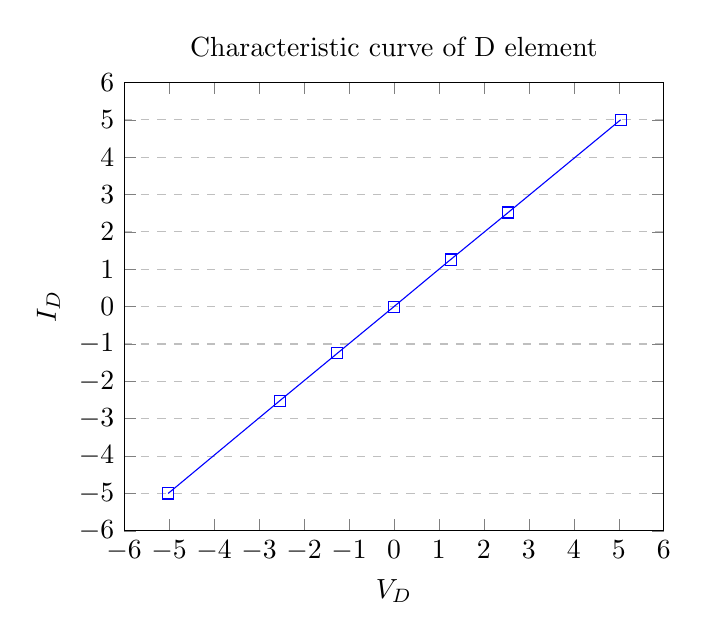
\begin{tikzpicture}
                    \begin{axis}[
                            title={Characteristic curve of D element},
                            xlabel={$V_D$},
                            ylabel={$I_D$},
                            xmin=-6, xmax=6,
                            ymin=-6, ymax=6,
                            % 
                            xtick={-6,-5,-4,-3,-2,-1,0,1,2,3,4,5,6},
                            ytick={-6,-5,-4,-3,-2,-1,0,1,2,3,4,5,6},
                            legend pos=north west,
                            ymajorgrids=true,
                            grid style=dashed,
                        ]
                        \addplot[
                            color=blue,
                            mark=square,
                        ]
                        coordinates {
                                (-5.02,-5.00)
                                (-2.54,-2.52)
                                (-1.26,-1.25)
                                (0,0)
                                (1.26,1.26)
                                (2.54,2.52)
                                (5.04,5.00)
                            };
                    \end{axis}
                \end{tikzpicture}
            \end{figure}
        }
    \end{subquestion}

    %--------------------------------------------
    \begin{subquestion}{Repeat the previous part for a diode.}
        \answer{
            \begin{figure}[H]
                \centering
                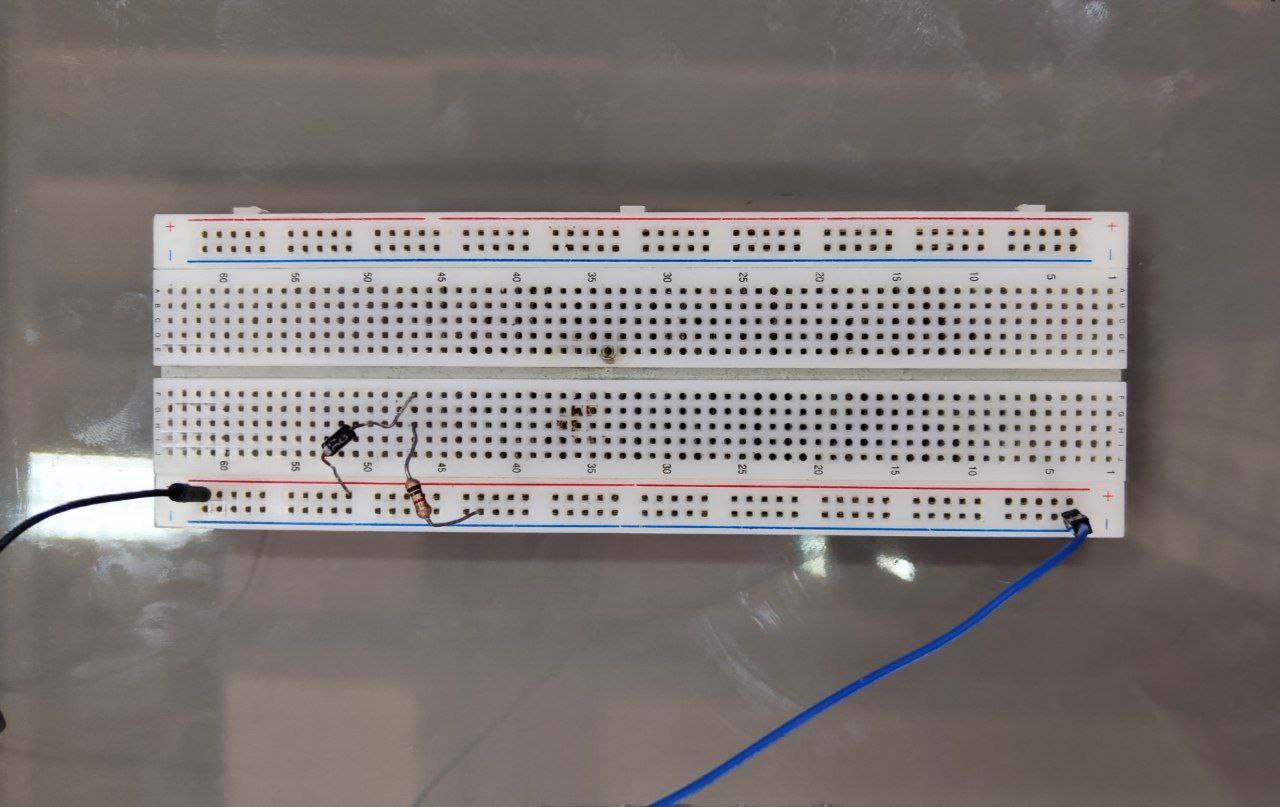
\includegraphics[scale=\PicScale,angle=0]{Fig/24.jpeg}
                \caption{The circuit.}
            \end{figure}

            \begin{figure}[H]
                \centering
                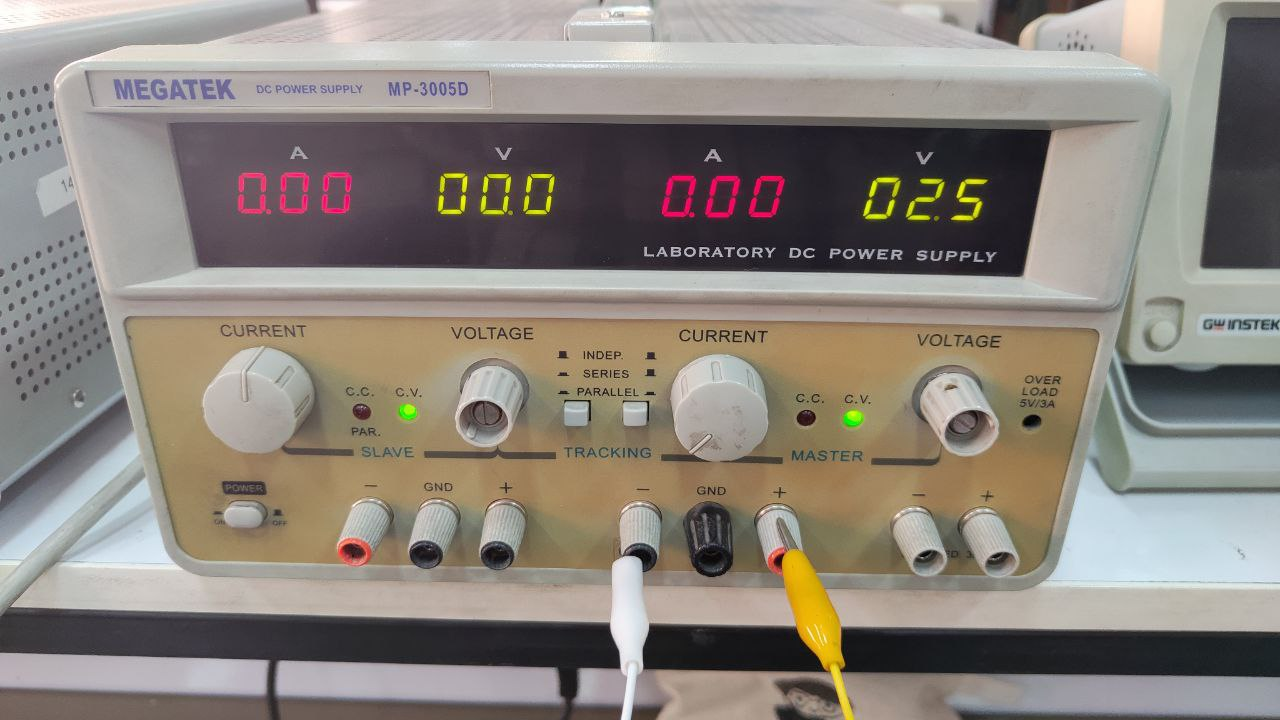
\includegraphics[scale=\PicScale,angle=0]{Fig/25.jpeg}
                \caption{DC power supply set to $10V$ and $-10V$.}
            \end{figure}
            \begin{figure}[H]
                \centering
                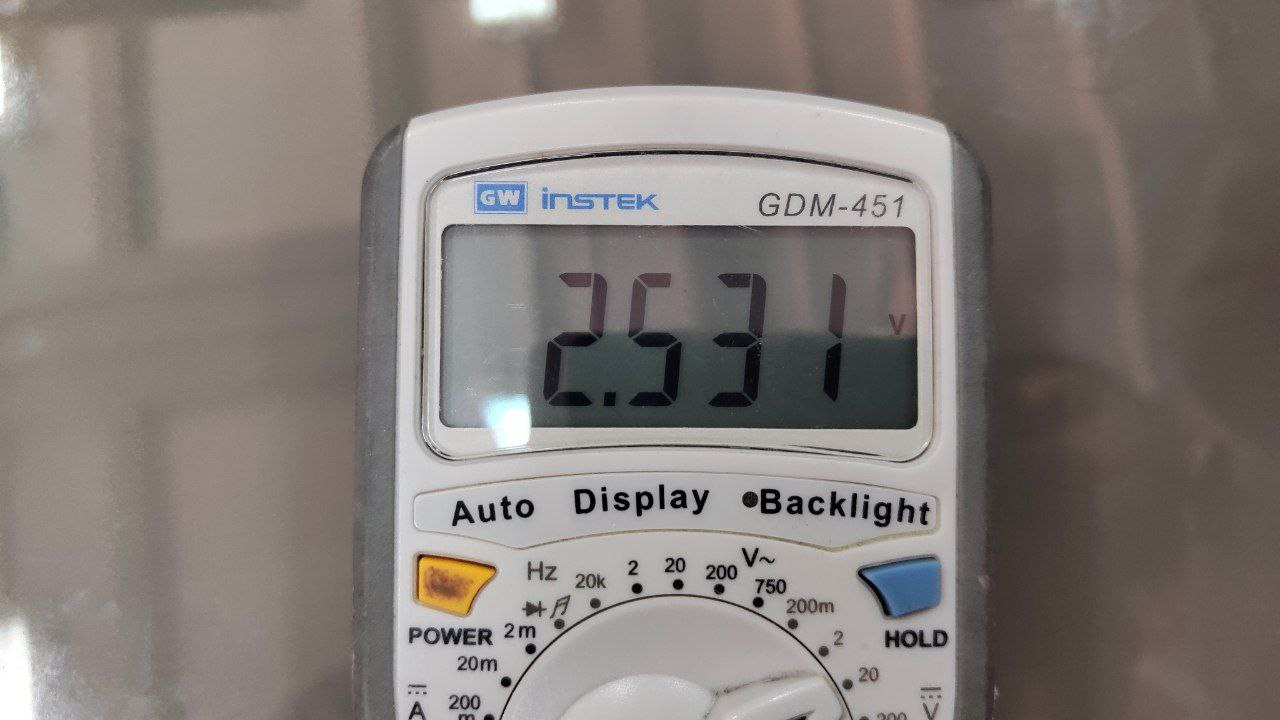
\includegraphics[scale=0.08,angle=0]{Fig/26.jpeg}
                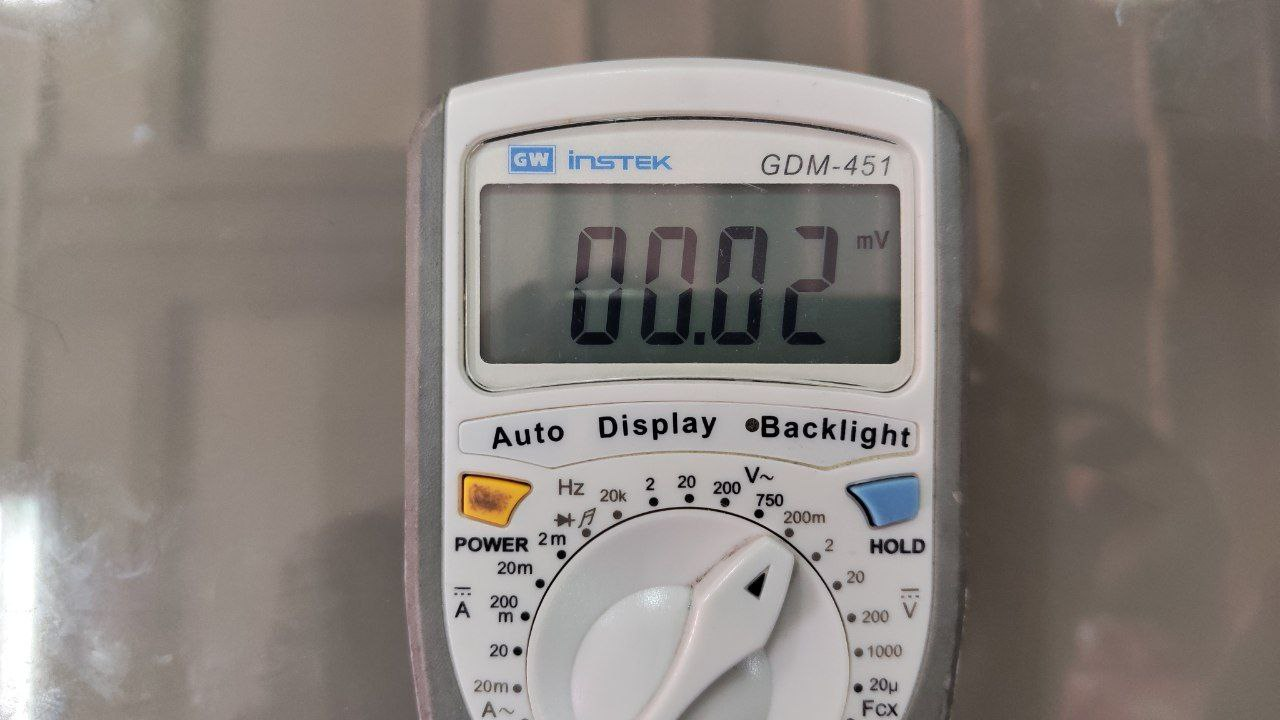
\includegraphics[scale=0.08,angle=0]{Fig/27.jpeg}
                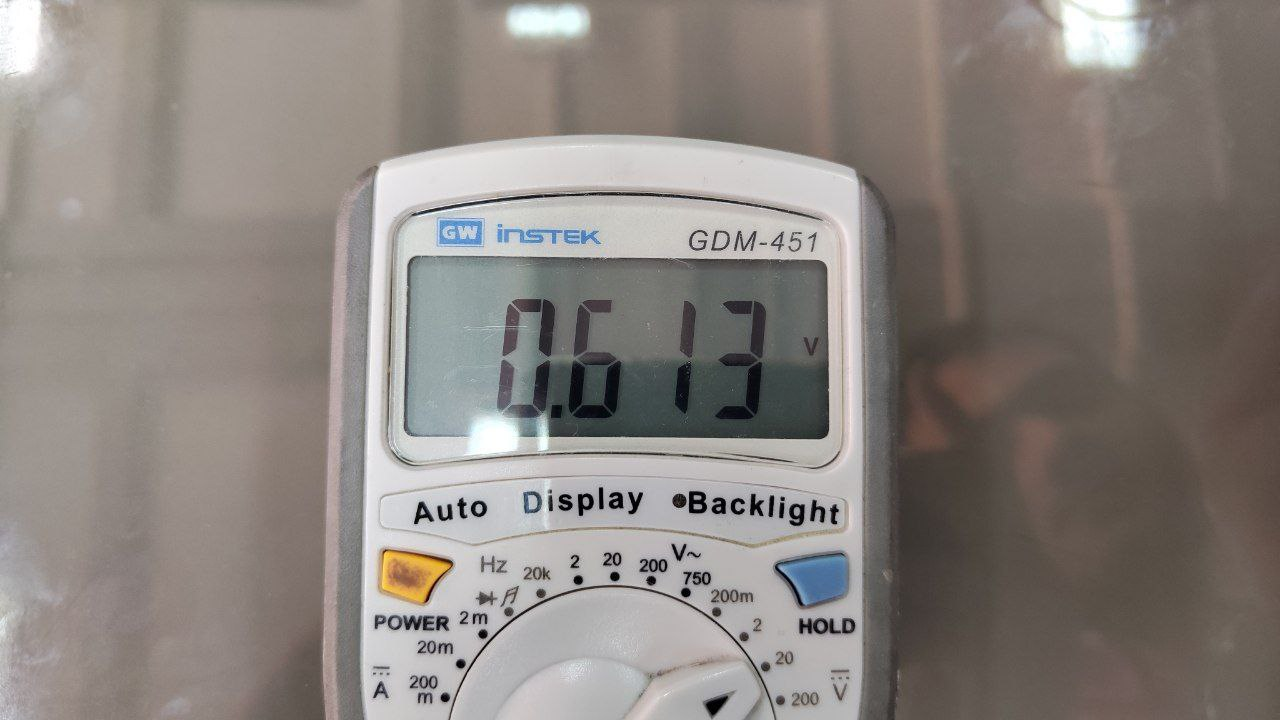
\includegraphics[scale=0.08,angle=0]{Fig/28.jpeg}
                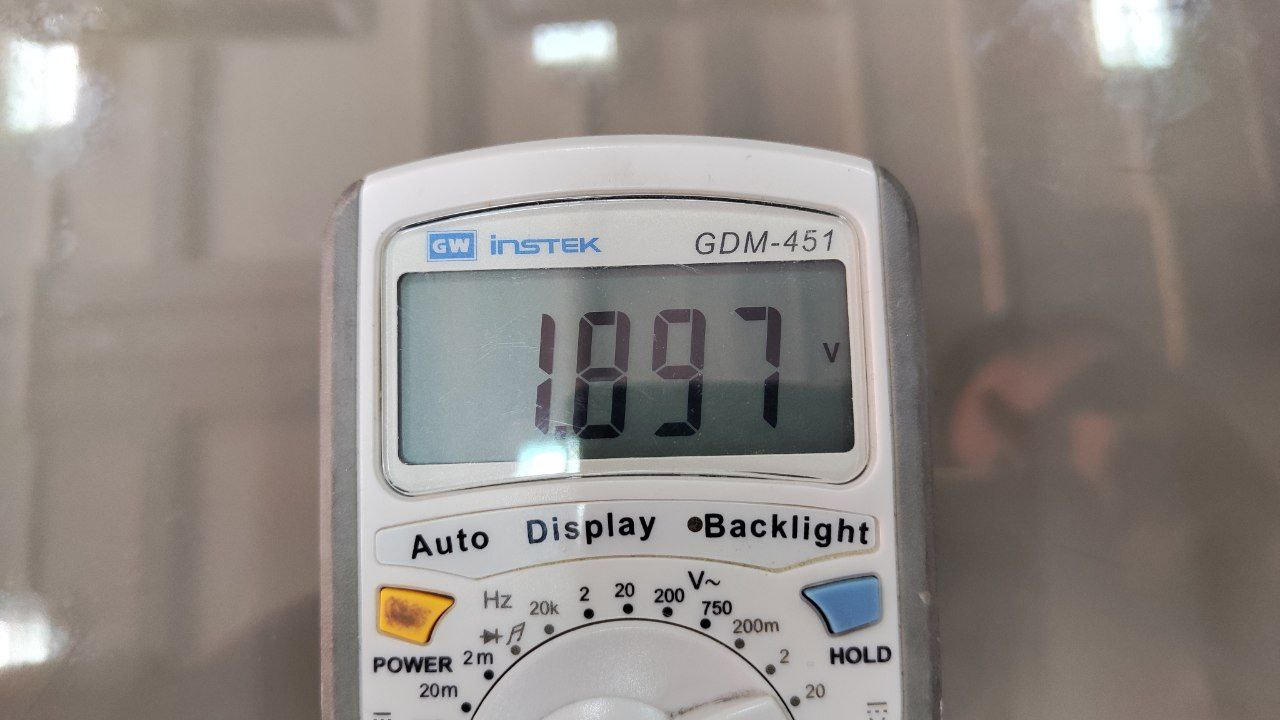
\includegraphics[scale=0.08,angle=0]{Fig/29.jpeg}
                \caption{First image is for D and $10V$, second image is for r and $10V$. \\
                    \hspace*{14mm} Third image is for D and $-10V$, last image is for r and $-10V$.}
            \end{figure}
            \begin{figure}[H]
                \centering
                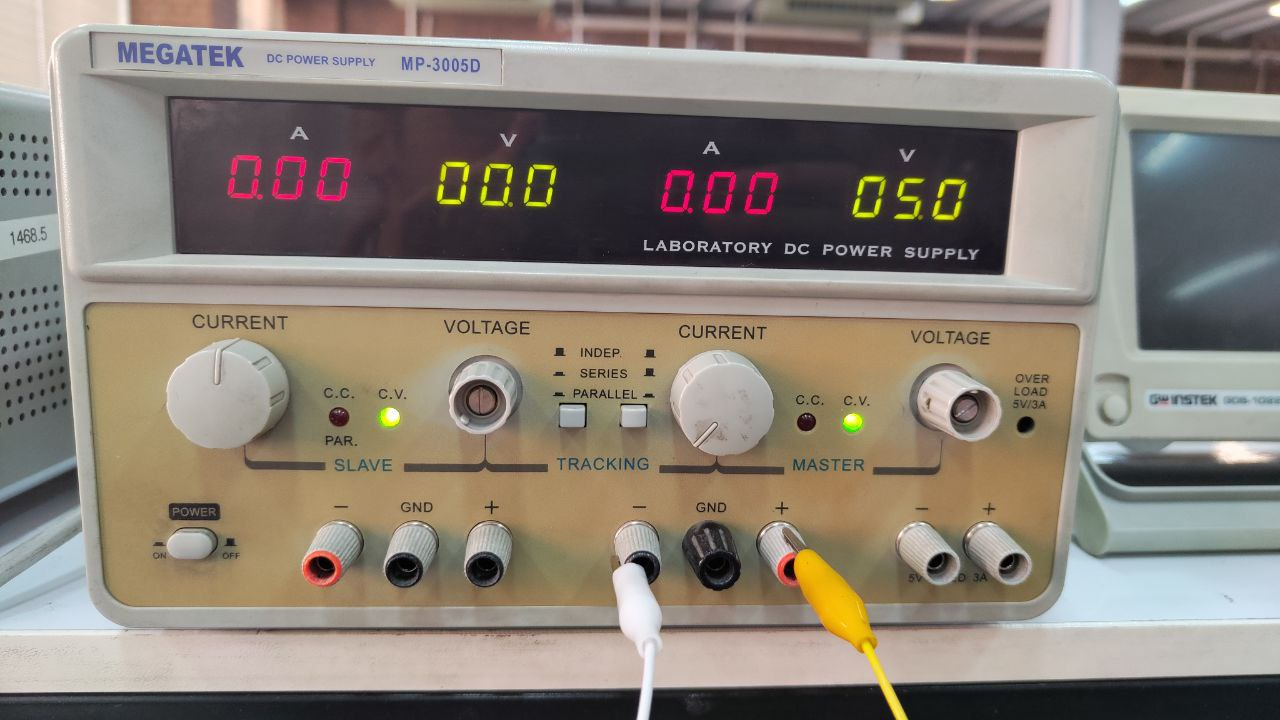
\includegraphics[scale=\PicScale,angle=0]{Fig/30.jpeg}
                \caption{DC power supply set to $5V$ and $-5V$.}
            \end{figure}
            \begin{figure}[H]
                \centering
                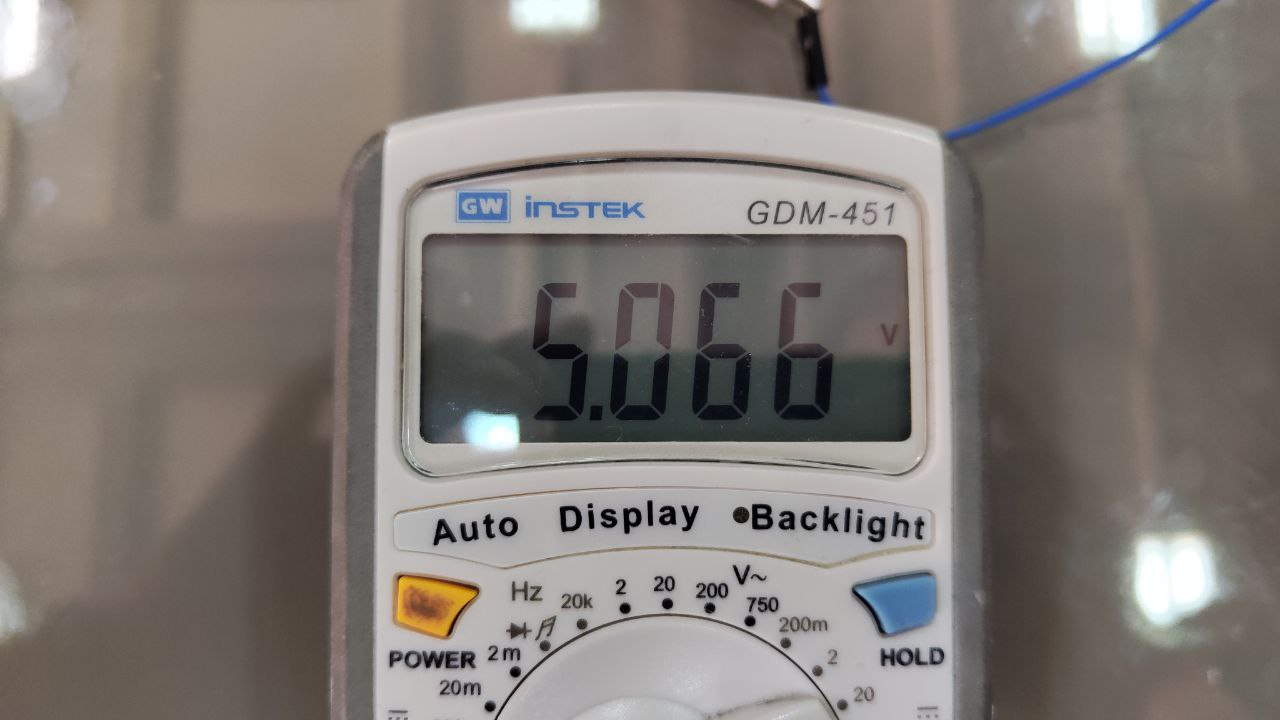
\includegraphics[scale=0.08,angle=0]{Fig/31.jpeg}
                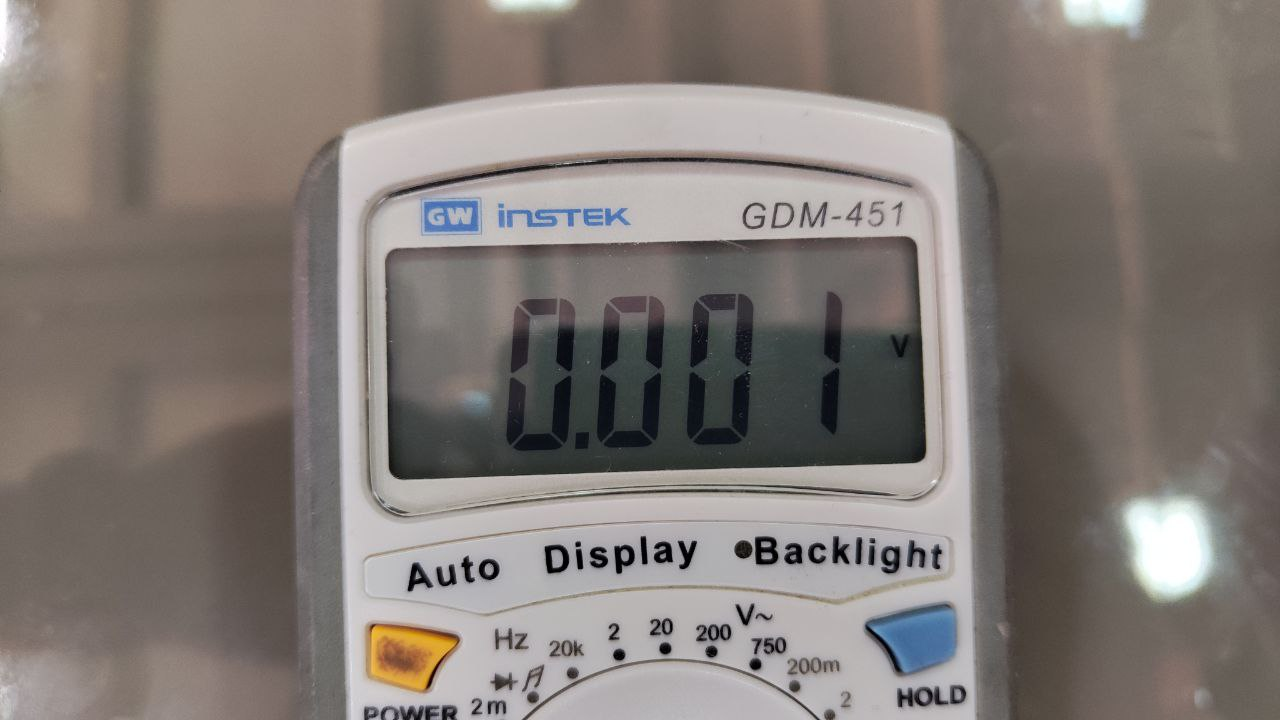
\includegraphics[scale=0.08,angle=0]{Fig/32.jpeg}
                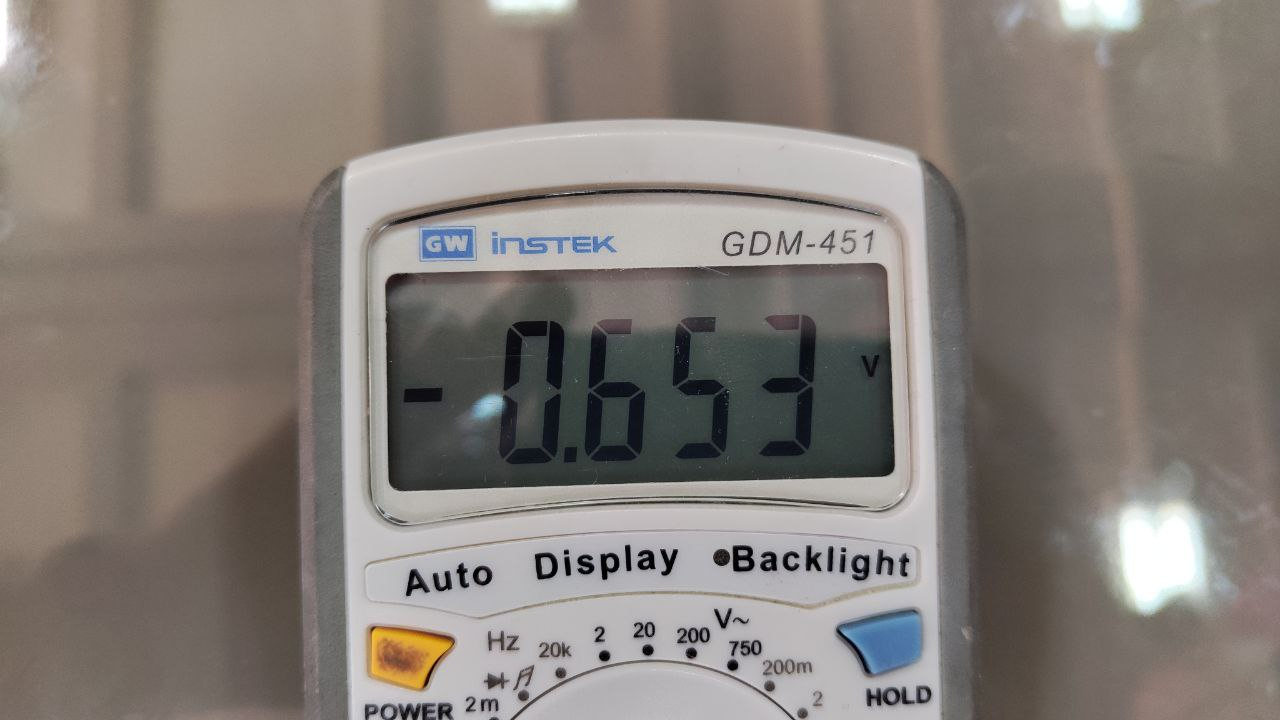
\includegraphics[scale=0.08,angle=0]{Fig/33.jpeg}
                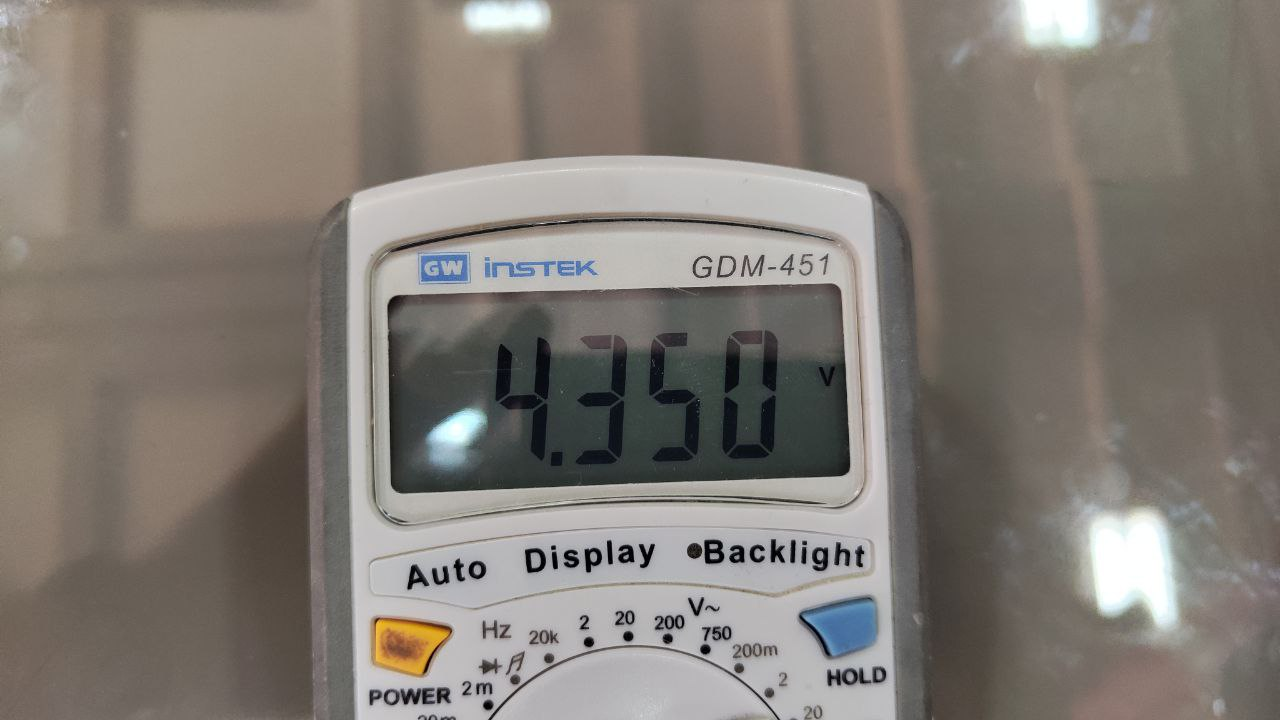
\includegraphics[scale=0.08,angle=0]{Fig/34.jpeg}
                \caption{First image is for D and $5V$, second image is for r and $5V$. \\
                    \hspace*{14mm} Third image is for D and $-5V$, last image is for r and $-5V$.}
            \end{figure}
            \begin{figure}[H]
                \centering
                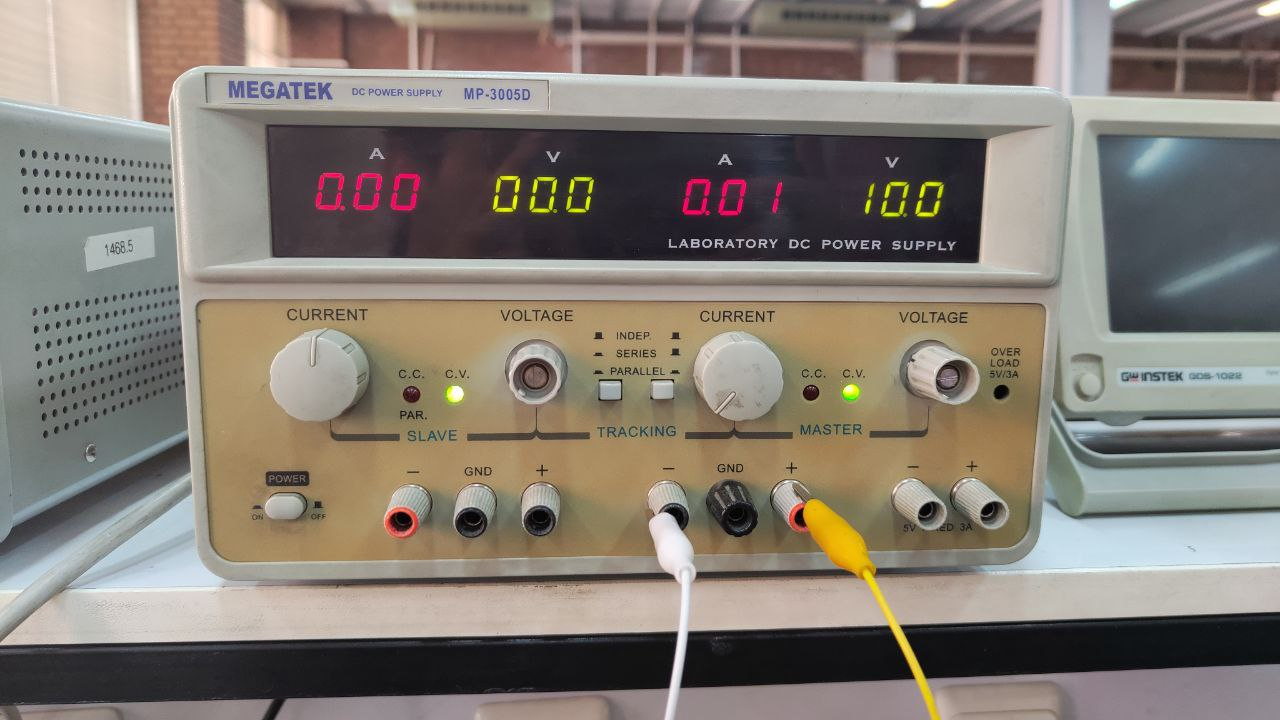
\includegraphics[scale=\PicScale,angle=0]{Fig/35.jpeg}
                \caption{DC power supply set to $2.5V$ and $-2.5V$.}
            \end{figure}
            \begin{figure}[H]
                \centering
                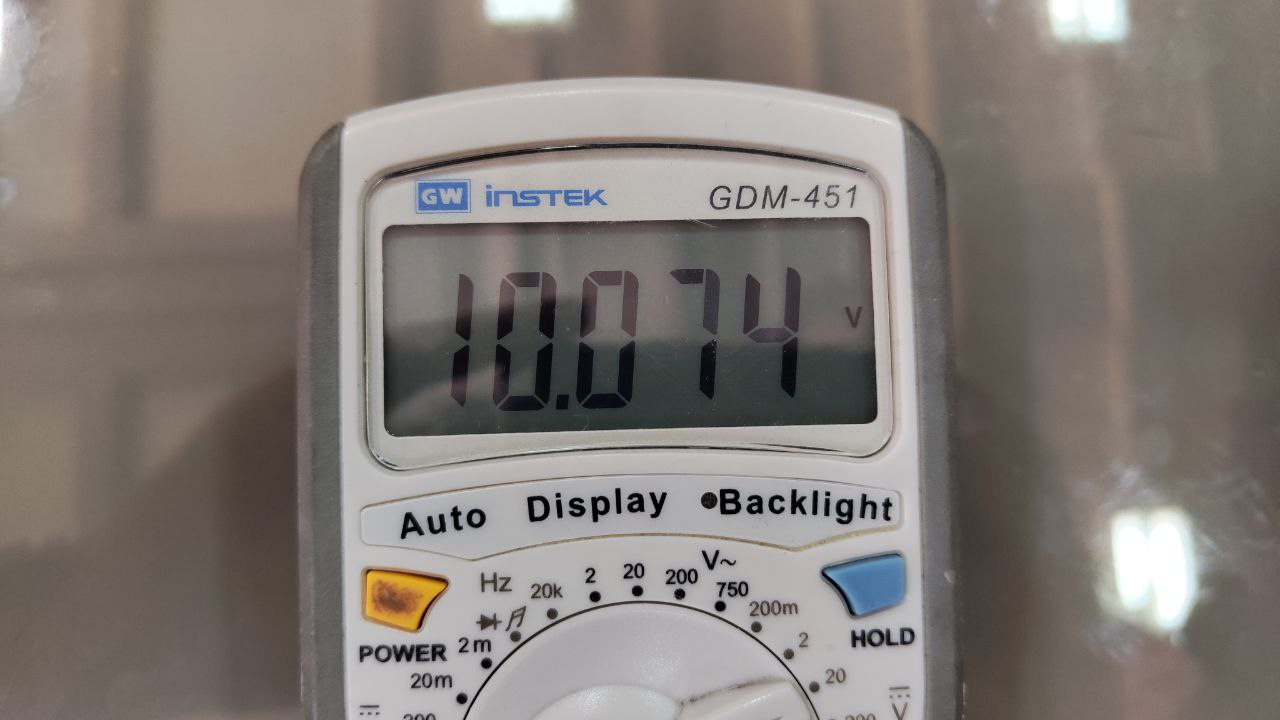
\includegraphics[scale=0.08,angle=0]{Fig/36.jpeg}
                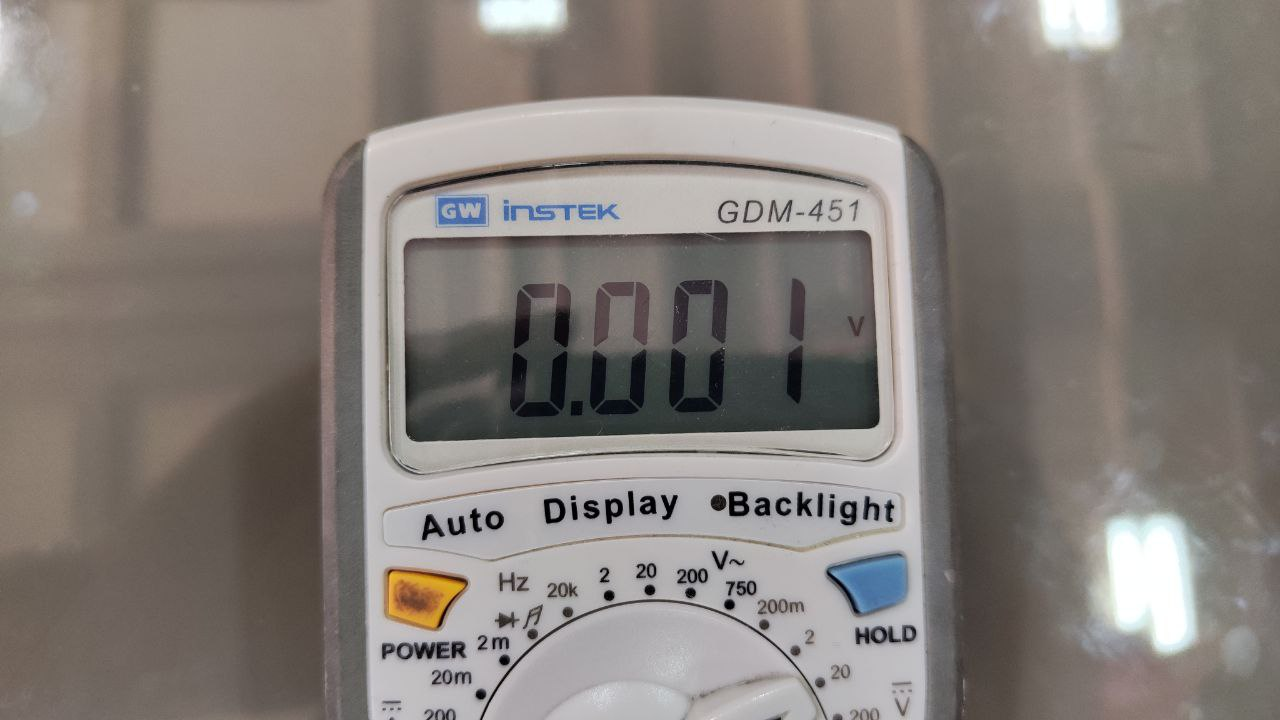
\includegraphics[scale=0.08,angle=0]{Fig/37.jpeg}
                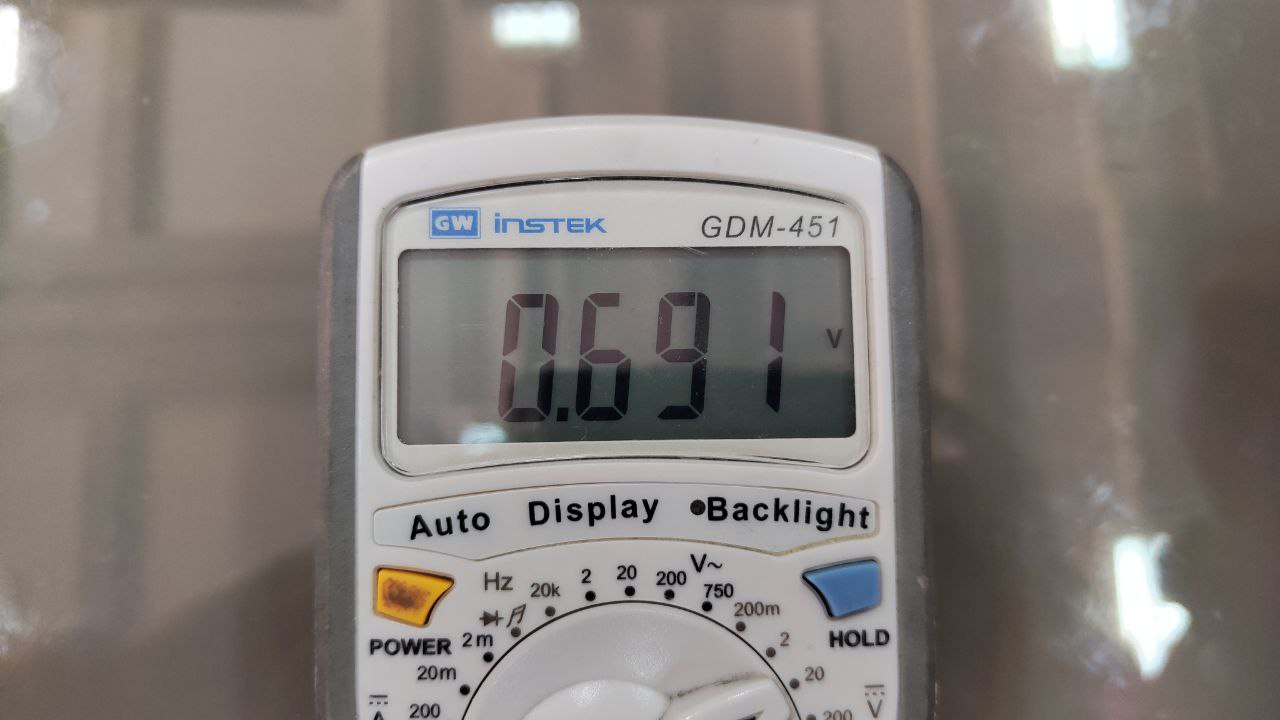
\includegraphics[scale=0.08,angle=0]{Fig/38.jpeg}
                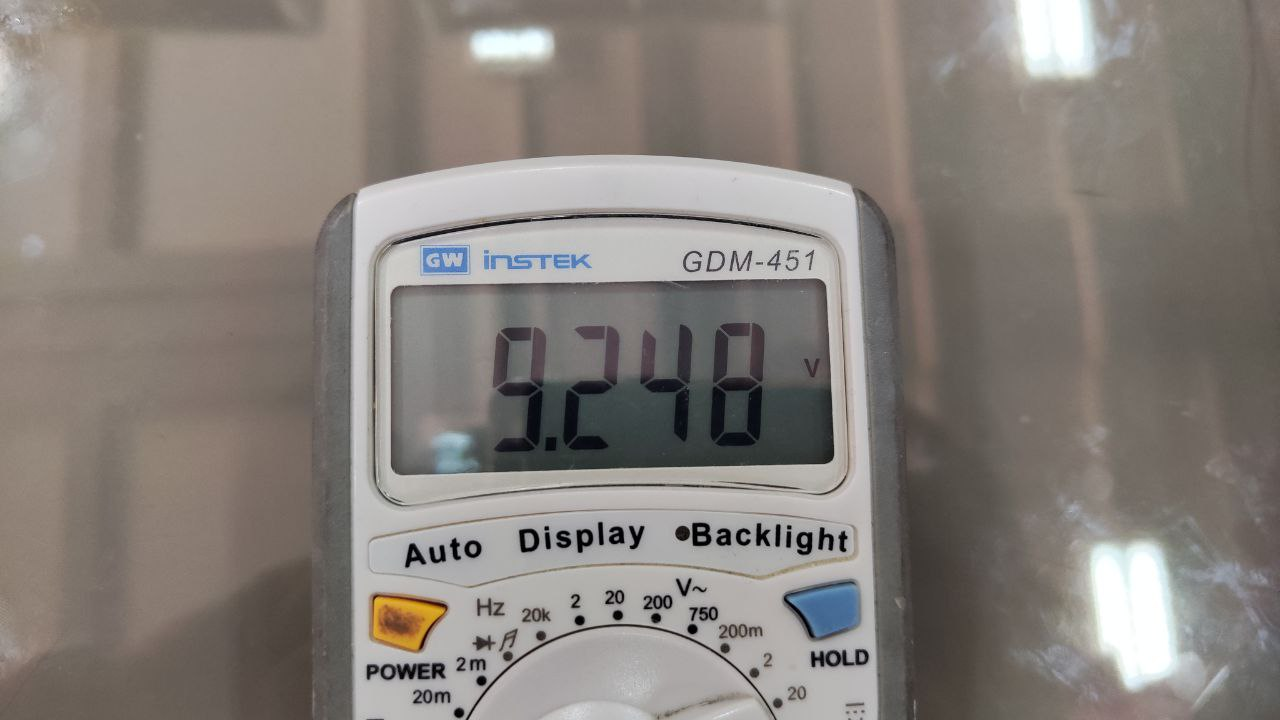
\includegraphics[scale=0.08,angle=0]{Fig/39.jpeg}
                \caption{First image is for D and $2.5V$, second image is for r and $2.5V$. \\
                    \hspace*{14mm} Third image is for D and $-2.5V$, last image is for r and $-2.5V$.}
            \end{figure}


            Similar to previous part, we can plot the characteristic curve of the D element in the
            same way.
            It will look like:
            \begin{figure}[H]
                \centering
                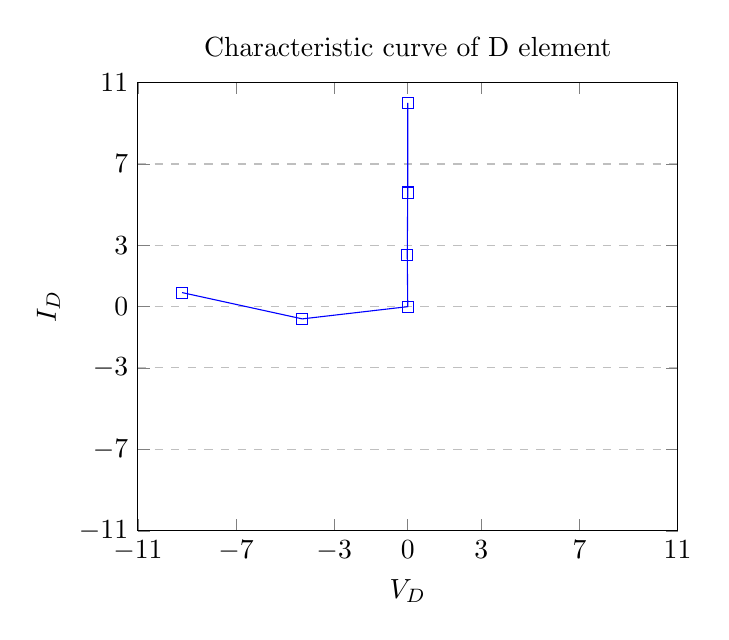
\begin{tikzpicture}
                    \begin{axis}[
                            title={Characteristic curve of D element},
                            xlabel={$V_D$},
                            ylabel={$I_D$},
                            xmin=-11, xmax=11,
                            ymin=-11, ymax=11,
                            % 
                            xtick={-11, -7 , -3, 0, 3, 7, 11},
                            ytick={-11, -7 , -3, 0, 3, 7, 11},
                            legend pos=north west,
                            ymajorgrids=true,
                            grid style=dashed,
                        ]
                        \addplot[
                            color=blue,
                            mark=square,
                        ]
                        coordinates {
                                (-9.2,0.69)
                                (-4.3,-0.6)
                                % (-1.89,0.6)
                                (0,0)
                                (-0.02,2.53)
                                (-0.001,5.6)
                                (-0.001,10.0)
                            };

                    \end{axis}
                \end{tikzpicture}
            \end{figure}

            % \begin{figure}[H]
            %     \centering
            %     % 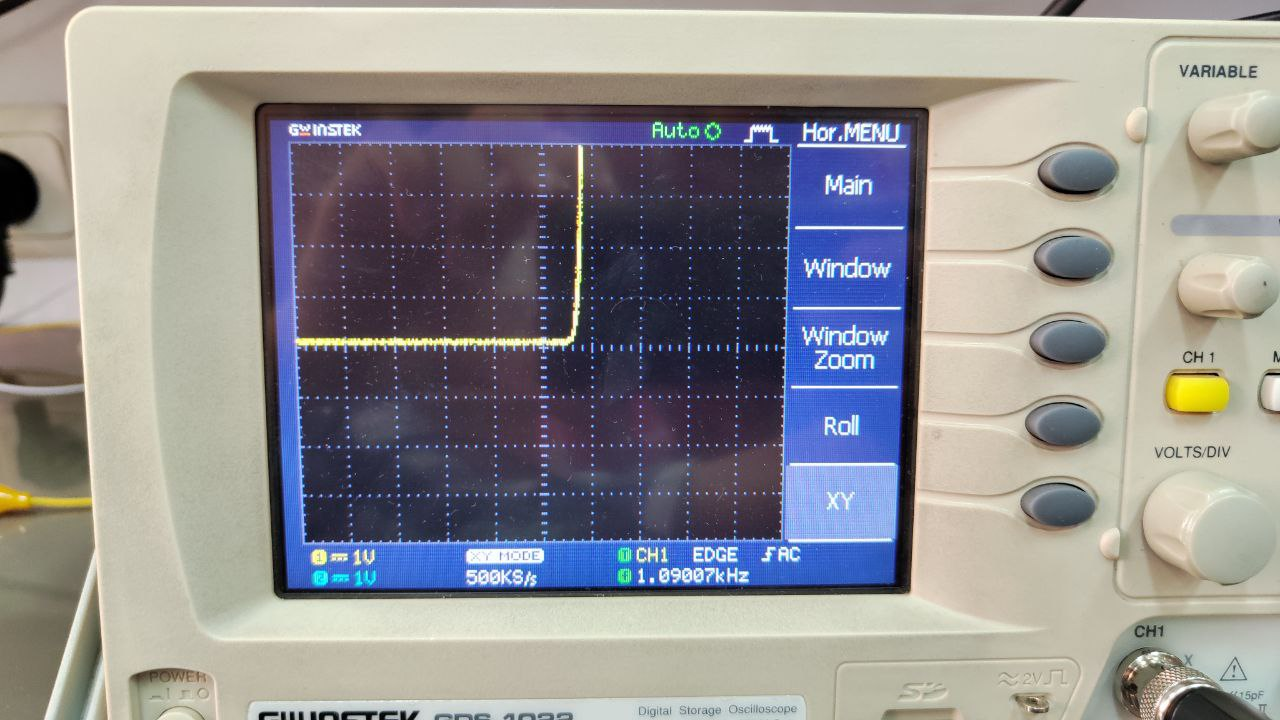
\includegraphics[scale=\PicScale,angle=0]{Fig/43.jpeg}
            %     % \caption{The oscilloscope showing diode characteristic curve.}
            % \end{figure}


        }
    \end{subquestion}


\end{question}


%----------------------------------------------------------------------------------------
%	QUESTION 1
%----------------------------------------------------------------------------------------

\begin{question}

    \questiontext{The experimental setup of Fig. \ref{fig:cir3} is used to display the Lissajous curve constructed by $v_x(t)$ and
        $v_y(t)$, where $D$ is a basic circuit element and $r=1$ k$\Omega$. }

    \begin{figure}[H]
        \centering
        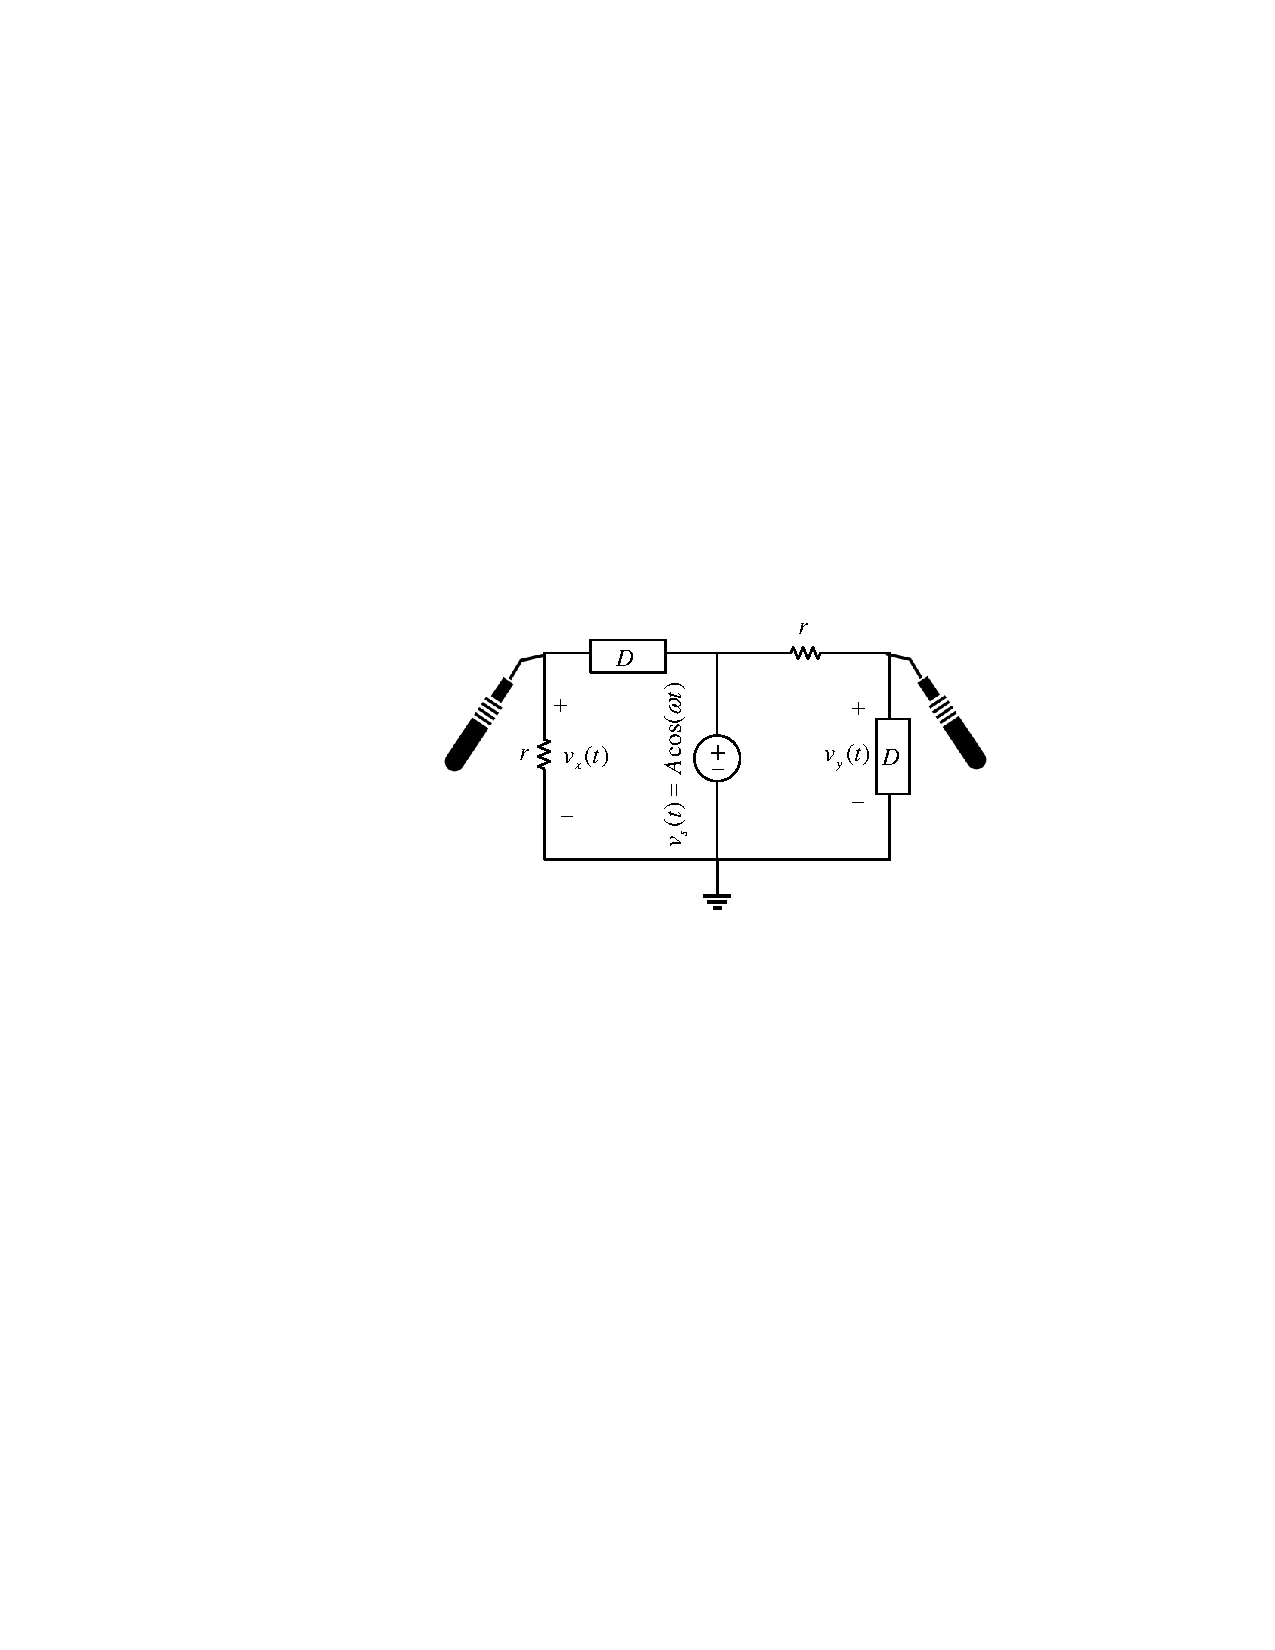
\includegraphics[scale=1.2,angle=0]{Fig/cir3.pdf}
        \caption{A test circuit for extracting the characteristic curve of a resistive element using oscilloscope.} \label{fig:cir3}
    \end{figure}

    % --------------------------------------------
    \begin{subquestion}{How can the displayed Lissajous curve be used
        to obtain the characteristic curve of a resistive element?}
    \answer{
        The Lissajous curve is a curve that is obtained by plotting the
        voltage of one element versus the voltage of another element.
        The slope of the curve is the ratio of the two voltages.
        The characteristic curve of a resistive element can be obtained by
        plotting the voltage of the resistive element versus
        the current flowing through it.In this circuit the first output
        shows the desired voltage of the element. Since the left side (resistor and D element)
        is parallel to the right side (resistor and D element), the right output
        is equivalent to the current flowing through the element.
        So the Lissajous curve can be used to obtain the characteristic
        curve of a resistive element.
    }
\end{subquestion}

%--------------------------------------------
\begin{subquestion}{Can the characteristic curve be extracted using the circuit of Fig. \ref{fig:cir2} and an oscilloscope? }
    \answer{
        yes, same as the previous question, if the value of
        the D element is equal to r resistor, the characteristic curve
        can be extracted using the circuit of Fig. \ref{fig:cir2} and an oscilloscope.
    }
\end{subquestion}

    \begin{subquestion}{Replace $D$ with a $1$ k$\Omega$ resistor and see the corresponding characteristic curve on the oscilloscope screen.}
        \answer{
            \begin{figure}[H]
                \centering
                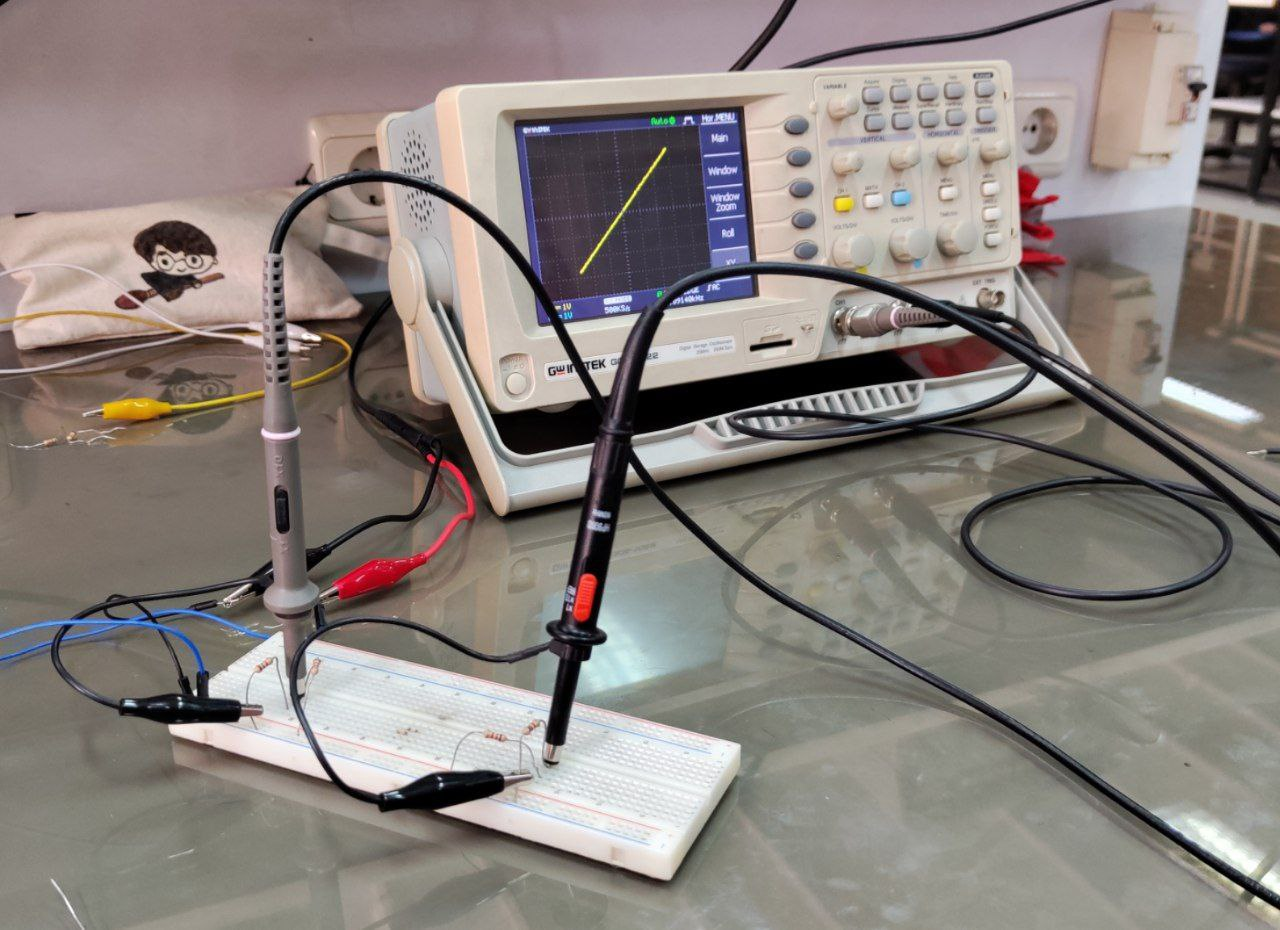
\includegraphics[scale=\PicScale,angle=0]{Fig/1000.jpeg}
                \caption{A photo of setup.}
            \end{figure}
            \begin{figure}[H]
                \centering
                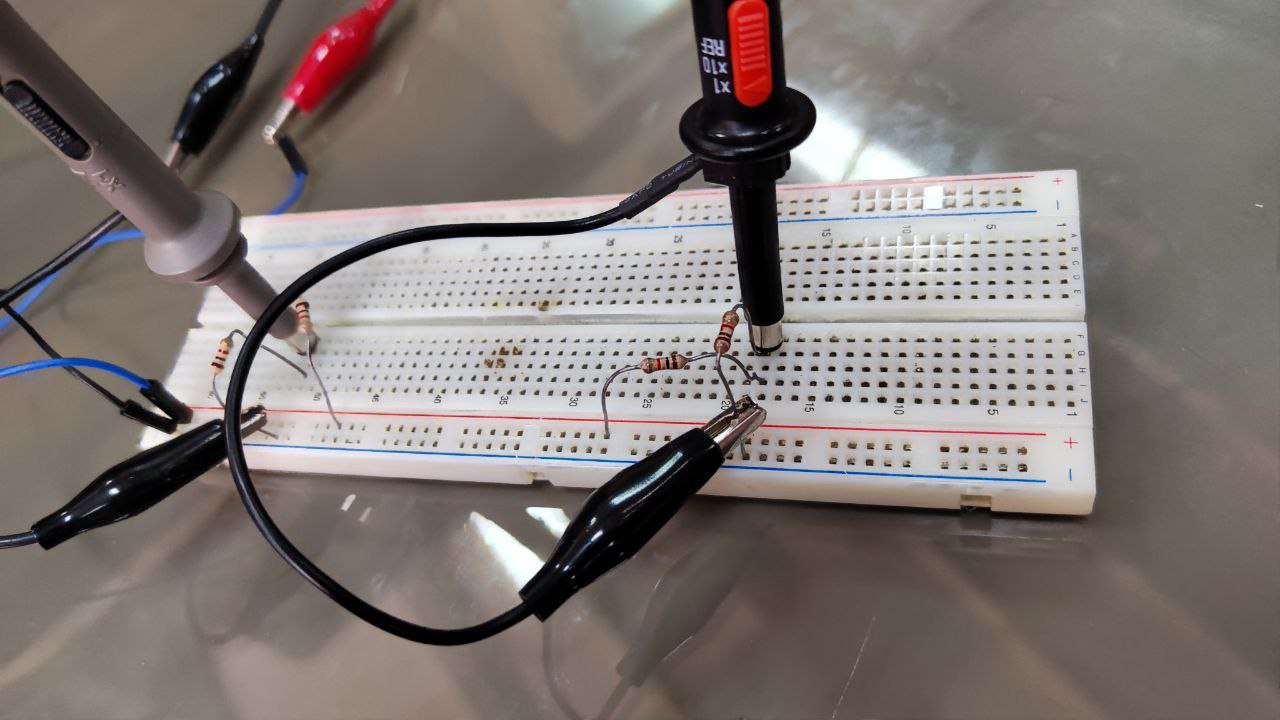
\includegraphics[scale=\PicScale,angle=0]{Fig/40.jpeg}
                \caption{The circuit.}
            \end{figure}
            \begin{figure}[H]
                \centering
                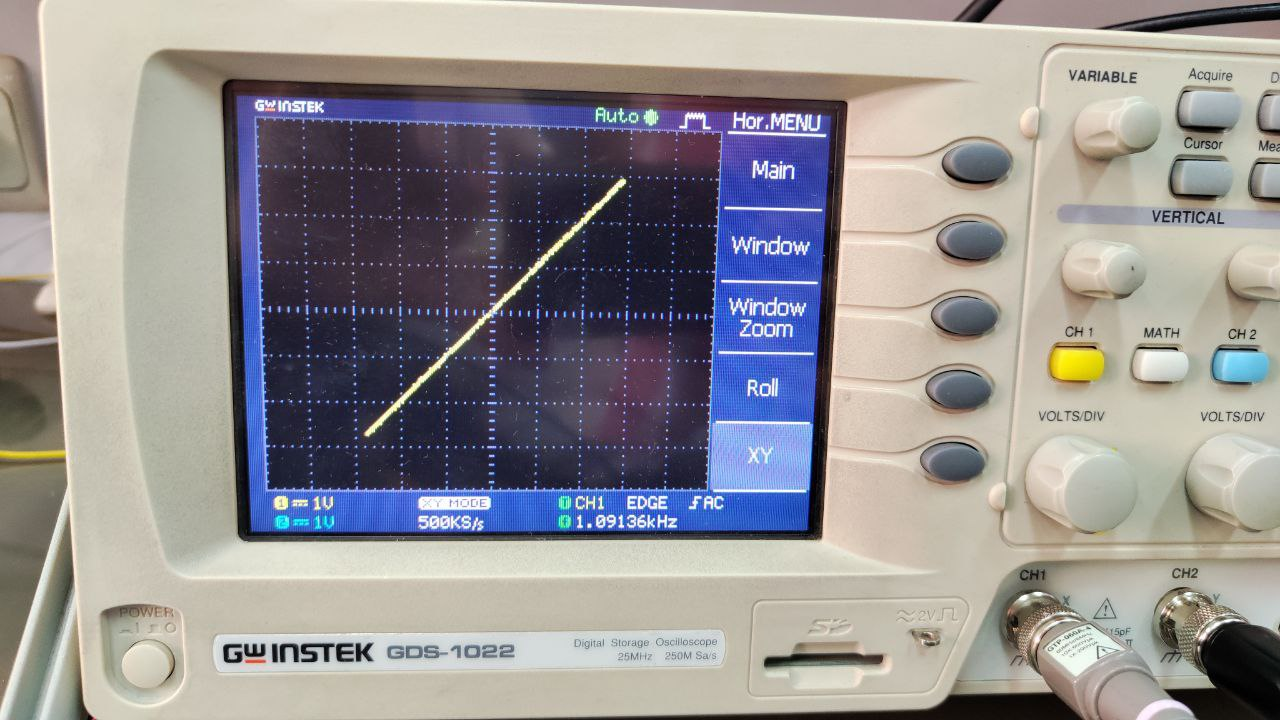
\includegraphics[scale=\PicScale,angle=0]{Fig/41.jpeg}
                \caption{The oscilloscope showing resistor characteristic curve.}
            \end{figure}
        }
    \end{subquestion}

    \begin{subquestion}{Repeat the previous part for a diode.}
        \answer{
            \begin{figure}[H]
                \centering
                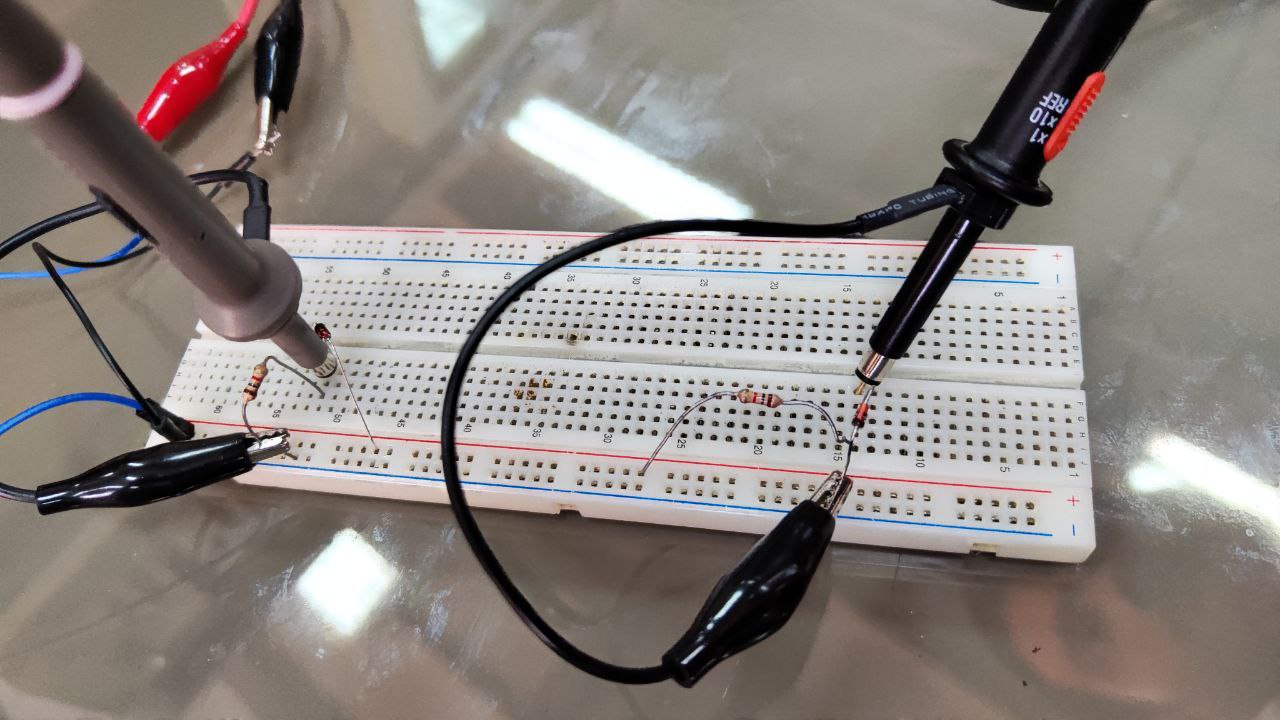
\includegraphics[scale=\PicScale,angle=0]{Fig/42.jpeg}
                \caption{The circuit.}
            \end{figure}
            \begin{figure}[H]
                \centering
                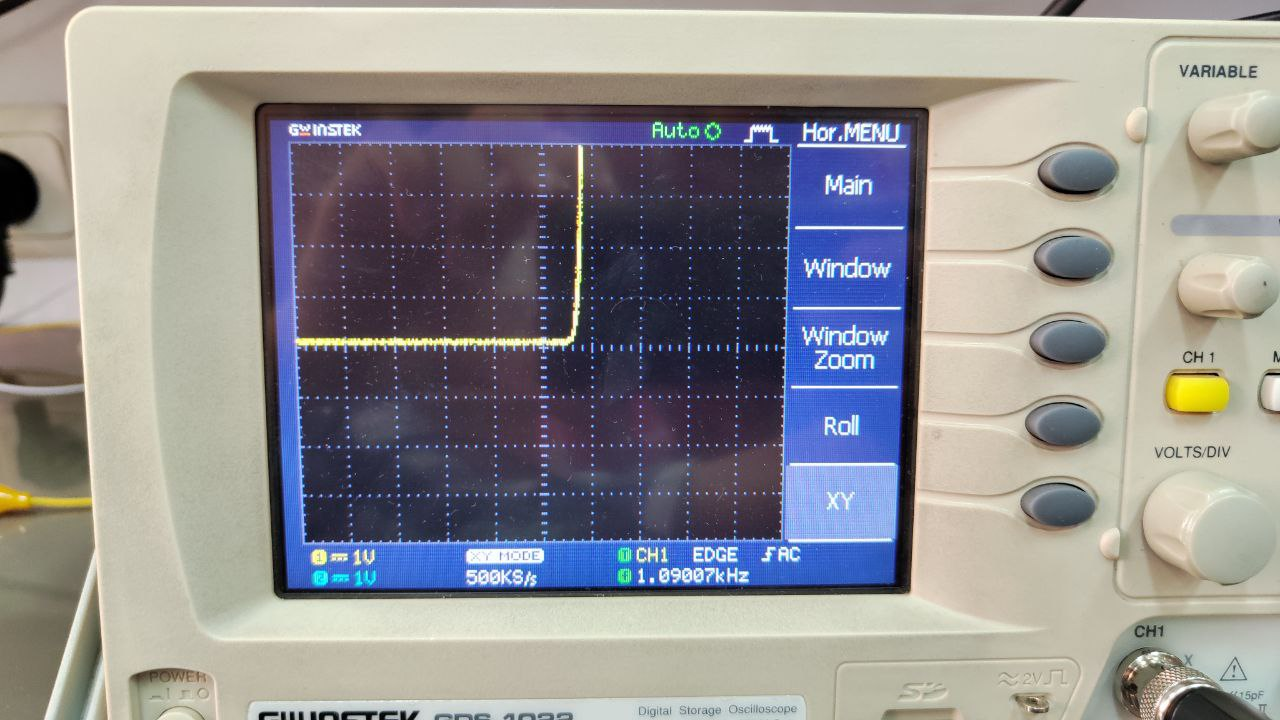
\includegraphics[scale=\PicScale,angle=0]{Fig/43.jpeg}
                \caption{The oscilloscope showing diode characteristic curve.}
            \end{figure}
        }
    \end{subquestion}


\end{question}

%----------------------------------------------------------------------------------------
%	QUESTION 1
%----------------------------------------------------------------------------------------

\begin{question}

    \questiontext{Consider the real capacitor modeled in Fig. \ref{fig:cir4}. }

    \begin{figure}[H]
        \centering
        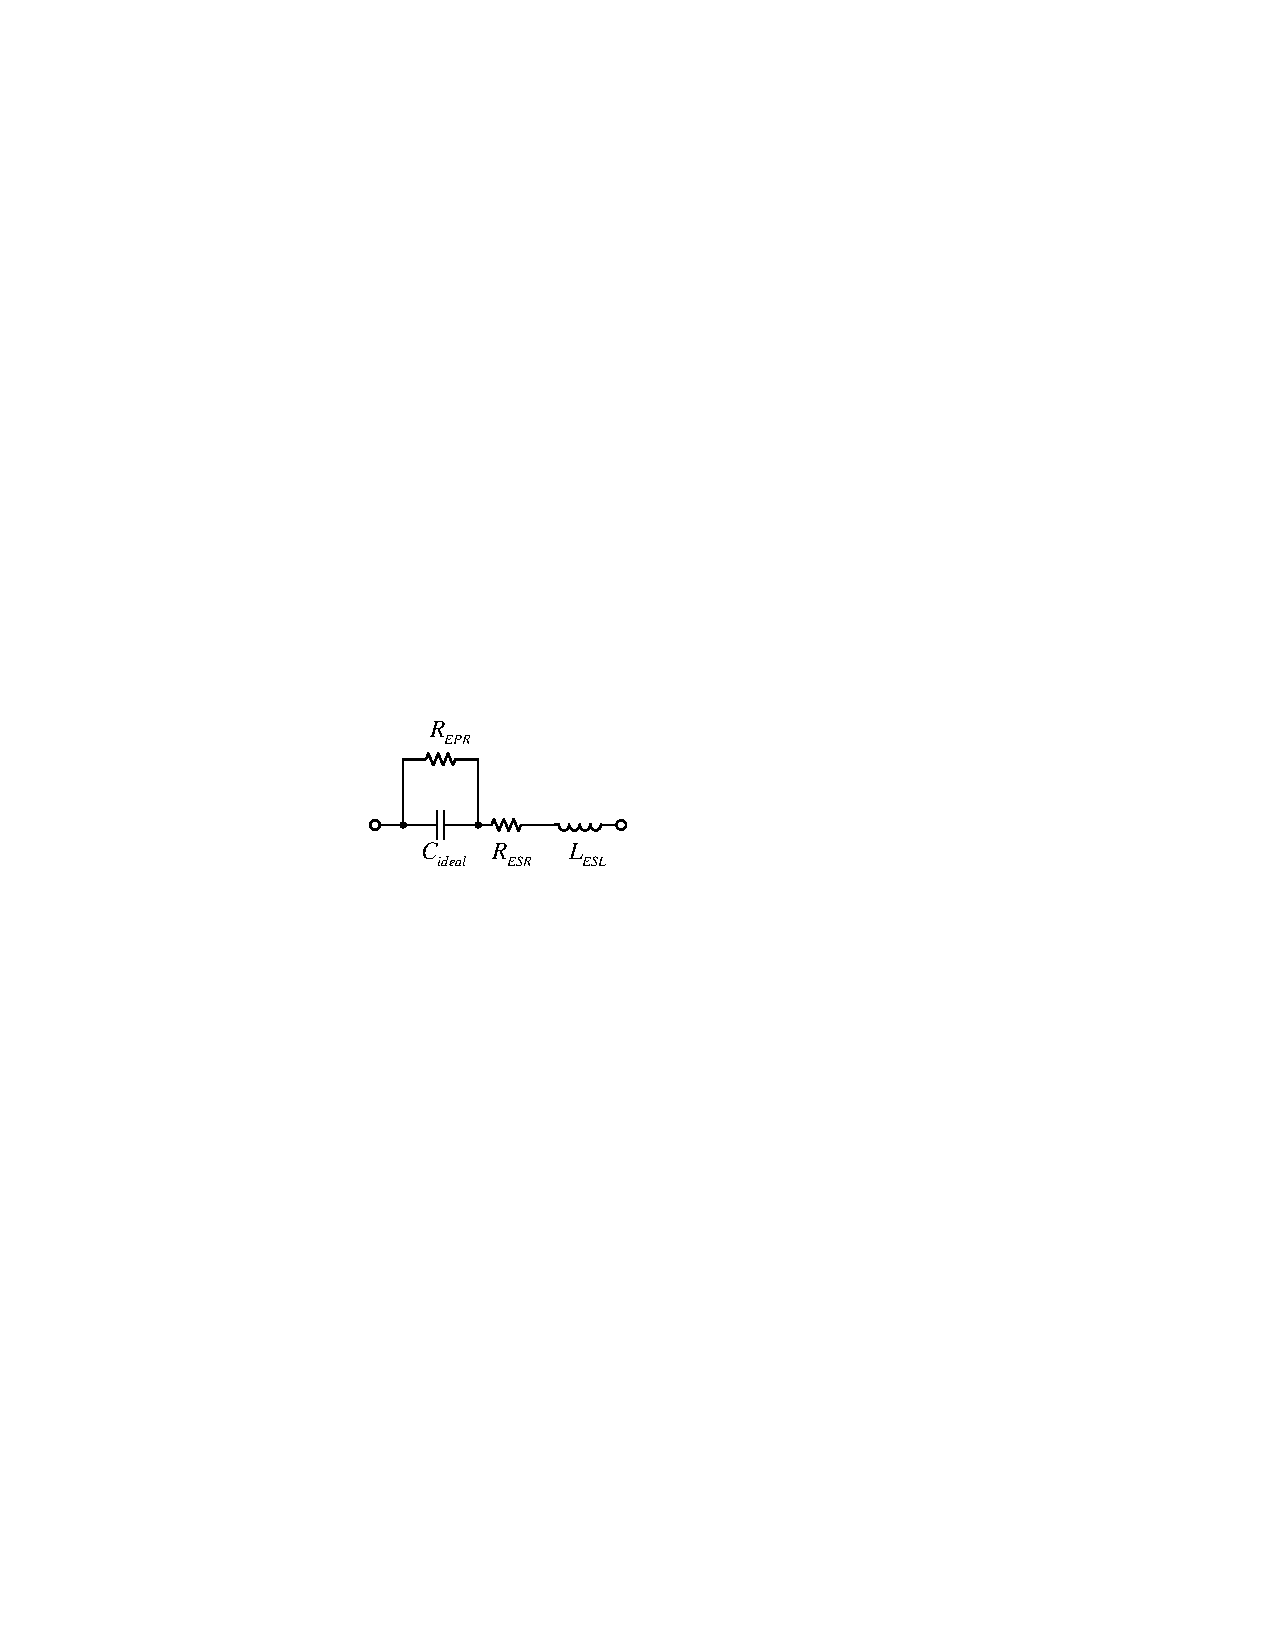
\includegraphics[scale=1.5,angle=0]{Fig/cir4.pdf}
        \caption{Real capacitor model.} \label{fig:cir4}
    \end{figure}

    %--------------------------------------------
    \begin{subquestion}{Assume that the sinusoidal voltage $v_C(t)=A\cos(\omega t+\theta)$ is applied to the capacitor. Find the corresponding capacitor current $i_C(t)$ for ideal values of $R_{EPR}$, $R_{ESR}$, and $L_{ESL}$ and show that it has sinusoidal form.}
        \answer{
            For an ideal capacitor, the current \( i_C(t) \) is related to the voltage \( v_C(t) \) by the equation:
            \[
                i_C(t) = C \frac{d v_C(t)}{dt}
            \]

            Given \( v_C(t) = A \cos(\omega t + \theta) \), we can find the derivative:
            \[
                \frac{d v_C(t)}{dt} = -A \omega \sin(\omega t + \theta)
            \]

            Substituting this derivative into the equation for \( i_C(t) \), we get:
            \[
                i_C(t) = C \frac{d v_C(t)}{dt} = -A \omega C \sin(\omega t + \theta)
            \]

            Using the trigonometric identity \( \sin(x) = \cos(x - \frac{\pi}{2}) \), we can rewrite the equation as:
            \[
                i_C(t) = -A \omega C \cos\left(\omega t + \theta - \frac{\pi}{2}\right)
            \]

            Therefore, the current \( i_C(t) \) has a sinusoidal form:
            \[
                i_C(t) = A \omega C \cos\left(\omega t + \theta - \frac{\pi}{2}\right)
            \]

        }
    \end{subquestion}

    %--------------------------------------------
    \begin{subquestion}{Use PSpice AC sweep analysis to plot the amplitude and phase of the capacitor current versus $f=\frac{\omega}{2\pi}$ when the capacitor voltage is $v_C(t)=\cos(\omega t+\theta)$ and $R_{EPR}$, $R_{ESR}$, and $L_{ESL}$ have ideal values.}
        \answer{

            Here is how the circuit looks like in PSpice:
            \begin{figure}[H]
                \centering
                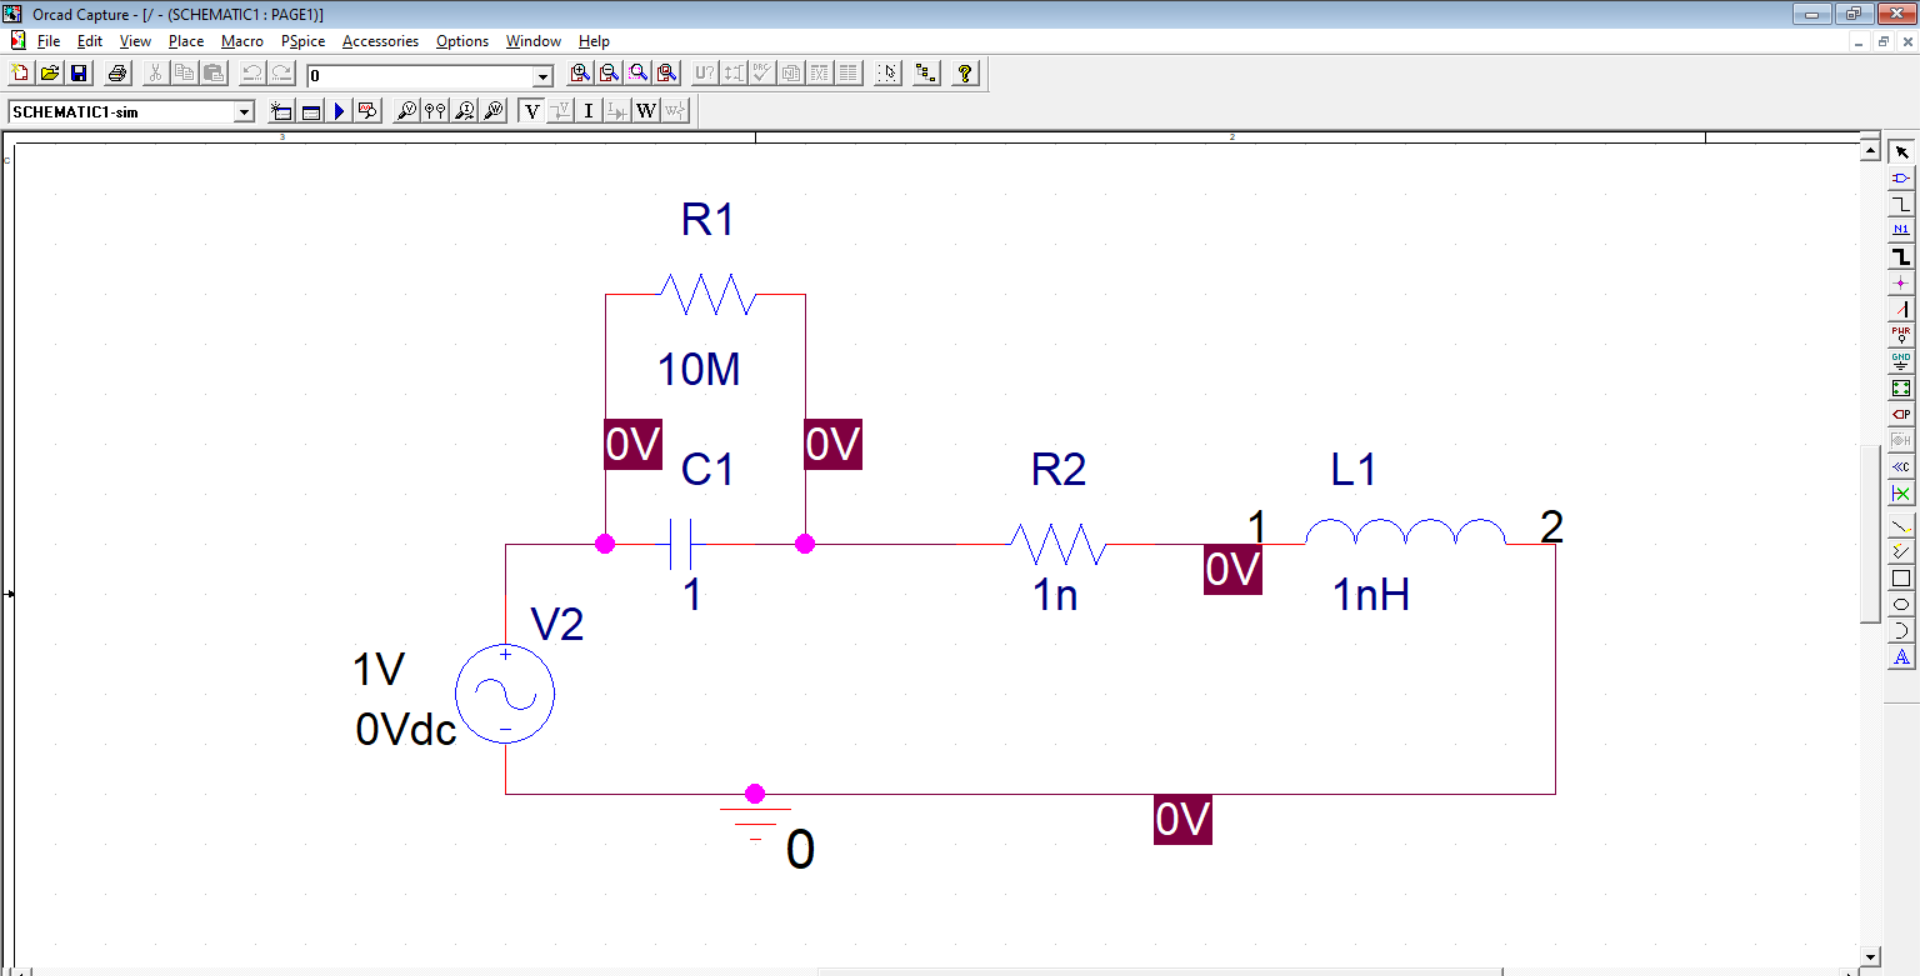
\includegraphics[scale=0.35,angle=0]{Fig/Q8.png}
                \caption{The circuit in PSpice.}
            \end{figure}

            The output of the simulation is:
            \begin{figure}[H]
                \centering
                \includegraphics[scale=0.35,angle=0]{Fig/Q8_1.png}
                \caption{The output of the simulation.}
            \end{figure}
        }
    \end{subquestion}

    %--------------------------------------------
    \begin{subquestion}{Use PSpice parametric analysis to plot the amplitude and phase of the capacitor current versus $f=\frac{\omega}{2\pi}$ for the capacitor voltage $v_C(t)=\cos(\omega t+\theta)$ and different suitably selected values of $R_{EPR}$, $R_{ESR}$, and $L_{ESL}$. Discuss how the parasitic parameters $R_{EPR}$, $R_{ESR}$, and $L_{ESL}$ affect the performance of the capacitor. }
        \answer{
            Here is how the circuit looks like in PSpice:
            \begin{figure}[H]
                \centering
                \includegraphics[scale=0.35,angle=0]{Fig/Q7_2.png}
                \caption{The circuit in PSpice.}
            \end{figure}

            The output of the simulation is:
            \begin{figure}[H]
                \centering
                \includegraphics[scale=0.35,angle=0]{Fig/Q7_3.png}
                \caption{The output of the simulation.}
            \end{figure}

            It can be observed that the parasitic parameters \( R_{EPR} \), \( R_{ESR} \), and \( L_{ESL} \) have a significant impact on the performance of the capacitor.
            These parasitic parameters introduce additional resistance and inductance to the circuit,
            which can affect the behavior of the capacitor.
            For example, the presence of resistance can lead to energy
            losses and reduce the efficiency of the capacitor.
            Similarly, the presence of inductance can introduce
            impedance to the circuit, affecting the current
            flow and the phase relationship between the voltage and current.
            Therefore, it is important to consider these parasitic parameters
            when designing and analyzing circuits involving capacitors to
            ensure optimal performance and accuracy.
        }
    \end{subquestion}

\end{question}

\assignmentSection{Bonus Experiments}

%----------------------------------------------------------------------------------------
%	QUESTION 8
%----------------------------------------------------------------------------------------
\begin{question}

    \questiontext{Write a MATLAB/Python code to plot the Lissajous curve corresponding to the voltage signals $v_x(t)=A_x\cos(\omega_x t+\theta_x)$ and $v_y(t)=A_y\cos(\omega_y t+\theta_y)$.}

    %--------------------------------------------
    \begin{subquestion}{Use the developed code to plot sample Lissajous curves for various values of $A_x$, $A_y$, $\omega_x$, $\omega_y$, $\theta_x$, and $\theta_y$. }
        \answer{

            The Matlab code:
            \lstinputlisting[style=Matlab-Pyglike]{code/one.m}

            The result of the code (for entries which are shown in the code):
            \begin{figure}[H]
                \centering
                \includegraphics[scale=0.8,angle=0]{Fig/Q7.png}
                \caption{The Lissajous curve.}
            \end{figure}


        }
    \end{subquestion}

    %--------------------------------------------
    \begin{subquestion}{Assume that $\frac{\omega_x}{\omega_y}=\frac{m}{n}$, where $\frac{m}{n}$ is a fractional number. Discuss how the ratio $\frac{\omega_x}{\omega_y}$ can be found from the corresponding Lissajous curve?}
        \answer{
            When the ratio of the angular frequencies, \(\frac{\omega_x}{\omega_y}\), is a fractional number, the resulting Lissajous curve provides a visual representation of this ratio. The Lissajous curve is formed by plotting the voltage signals \(v_x(t)\) and \(v_y(t)\) as a parametric curve in the xy-plane.

            Specifically, when \(\frac{\omega_x}{\omega_y} = 1\), the Lissajous curve takes the shape of an ellipse. This ellipse can degenerate
            into a line when the phase difference
            between the two signals, \(\theta_x - \theta_y\), is zero.

            When \(\frac{\omega_x}{\omega_y} = 2\), the Lissajous
            curve forms a figure-eight pattern. This pattern occurs
            when the two signals have a phase difference
            of \(\frac{\pi}{2}\).

            In general, for \(\frac{\omega_x}{\omega_y} = \frac{m}{n}\),
            where \(m\) and \(n\) are integers, the Lissajous
            curve will have \(m\) horizontal lobes and \(n\)
            vertical lobes. The lobes represent the number of
            times the curve intersects the x-axis and y-axis,
            respectively.

            By visually inspecting the Lissajous curve and
            counting the number of lobes, one can determine
            the ratio \(\frac{\omega_x}{\omega_y}\) and gain
            insights into the relationship between the two signals.
        }
    \end{subquestion}

\end{question}


%----------------------------------------------------------------------------------------
%	QUESTION 10
%----------------------------------------------------------------------------------------

\begin{question}

    \questiontext{Return your work report by filling the \LaTeX template of the manual. Include useful and high-quality images to make the report more readable and understandable.}

\end{question}

%----------------------------------------------------------------------------------------

\end{document}
